\typeout{(body.tex)}

\begin{frame}
    \titlepage
\end{frame}

\begin{frame}{lectures}
    \begin{itemize}
    \item I will audio+screenrecord my lectures
        \begin{itemize}
        \item intend to find a way to post them later in the same day
        \item suggest VLC for viewing (supports changing speed!)
        \end{itemize}
    \item lecture attendence is strongly recommended, but \ldots
    \item I won't check
    \end{itemize}
\end{frame}

\begin{frame}{different lecturers?}
    \begin{itemize}
    \item Mark Floryan also teaches this class
    \item we are giving seperate lectures
    \item different slidedecks
        \begin{itemize}
        \item but similar
        \item I made my slides by looking at Floryan's\ldots
        \item (but have some different preferences/style than him\ldots)
        \end{itemize}
    \end{itemize}
\end{frame}

\begin{frame}{homeworks (AKA labs)}
    \begin{itemize}
    \item weekly assignments with three parts:
    \vspace{.5cm}
    \item \textit{pre-lab} due Tuesday morning
    \item \textit{in-lab} done \myemph{physically in the lab section you are registered for}
    \item \textit{post-lab} due Friday morning
    \end{itemize}
\end{frame}

\begin{frame}{course staff}
    \begin{itemize}
        \item lecturers: Mark Floryan and I
        \item more than 20 TAs
        \item some graduate student graders
    \end{itemize}
\end{frame}

\begin{frame}{questions}
    \begin{itemize}
    \item Piazza 
    \item support request tool
        \begin{itemize}
        \item linked off website
        \item preferred way to contact faculty
        \end{itemize}
    \item office hours (faculty and TA)
        \begin{itemize}
        \item Google calendar linked off website
        \end{itemize}
    \end{itemize}
\end{frame}

\begin{frame}{announcements}
    \begin{itemize}
    \item course twitter feed --- \texttt{@UVaCS2150}
        \begin{itemize}
            \item shown on Collab
        \end{itemize}
    \item emails to class --- very sparingly
    \end{itemize}
\end{frame}

\begin{frame}{prerequisites}
    \begin{itemize}
        \item C- or better in CS2110 or CS 2220
            \begin{itemize}
            \item references, classes, objects, generics (or templates)
            \item control structures, procedures, recursion
            \item writing programs longer than a screenful
            \end{itemize}
        \item C- or better in CS2102
            \begin{itemize}
            \item logarithms, sets, graphs
            \item proof techniques, including by contradiciton
            \end{itemize}
    \end{itemize}
\end{frame}

\begin{frame}{CS2102 as co-requisite}
    \begin{itemize}
        \item you may take CS2102 as a co-requisite instead
        \item but \myemph{at your own risk}
        \item we may ask exam questions that require CS2102 material
    \end{itemize}
\end{frame}

\begin{frame}{lab swapping}
    \begin{itemize}
    \item no, we cannot 
    \begin{itemize}
        \item change lab you are enrolled in ourselves
        \item increase lab capacities beyond 45 (fire marshall limits)
        \end{itemize}
    \item to switch to an \textit{open} lab, you can use ``Edit Class'' in SIS
        \begin{itemize}
        \item do not drop the course and readd (you may end up on the waitlist)
        \end{itemize}
    \item if you and another student want to swap labs, \\
          Engineering main office in Thornton A122 may be able to do this
        \begin{itemize}
        \item you can try to find students to do this with on Piazza
        \end{itemize}
    \end{itemize}
\end{frame}

\begin{frame}{honor-related policies}
    \begin{itemize}
    \item do \textbf{not} share your code 
    \item do \textbf{not} look at another student's code
    \item do \textbf{not} try to hack the submission system
    \item do \textbf{not} share midterm details with students who haven't taken it yet
    \item \myemph<2>{do \textbf{not} release your source code online}\tikzmark{sourceOnline}
    \item \myemph<3>{when we ask for assembly files, do \textbf{not} submit\tikzmark{compAsm} compiler-generated} files unless otherwise allowed
    \end{itemize}
    \begin{tikzpicture}[overlay,remember picture]
        \begin{visibleenv}<2>
        \node[mycallout=sourceOnline] at ([yshift=-1.6cm,xshift=-4cm]pic cs:sourceOnline) {
            you \textbf{must not} do your work in a public github repo
        };
        \end{visibleenv}
    \end{tikzpicture}
    \begin{tikzpicture}[overlay,remember picture]
        \begin{visibleenv}<3>
        \coordinate (compAsmTop) at ([yshift=2ex]pic cs:compAsm);
        \node[mycallout2=compAsmTop,align=left] at ([yshift=1.5cm,xshift=-8cm]compAsmTop) {
            probably the lab is about writing assembly, \\ \textbf{not} using compilers\ldots
        };
        \end{visibleenv}
    \end{tikzpicture}
\end{frame}

\begin{frame}{academic honesty}
    \begin{itemize}
    \item we will refer to honor violations/cheating to the honor commitee
    \item we will also give you an F in the course for them
    \end{itemize}
\end{frame}

\begin{frame}{grading}
    \begin{itemize}
    \item 45\% labs
    \item 30\% midterms --- in lab!
    \item 25\% final exam
    \end{itemize}
\end{frame}

\begin{frame}{late policy}
    \begin{itemize}
    \item see \href{https://markfloryan.github.io/pdr/uva/labduedates.html}{discussion} linked from first lab
        \begin{itemize}
            \item summary (1): -25\% for first 24 hours
            \item summary (2): you can request an extension for any in-lab
        \end{itemize}
        \vspace{.5cm}
    \item lab due times are strictly enforced
    \end{itemize}
\end{frame}

\begin{frame}{compilation}
    \begin{itemize}
    \item does not compile = \myemph{no credit}
        \begin{itemize}
        \item copy and paste error? we are not going to fix it
        \end{itemize}
    \vspace{.5cm}
    \item the lab submission tells you if it compiles
    \end{itemize}
\end{frame}

\begin{frame}{final exam}
    \begin{itemize}
    \item 7 May at 7PM
    \item tell us if you have a conflict \textit{this month}
        \begin{itemize}
        \item via support request link in git repo (later)
        \end{itemize}
    \item conflict = cannot attend the exam
        \begin{itemize}
        \item (e.g. another exam at same time)
        \item exams at other times on 7 May is not a conflict
        \end{itemize}
    \end{itemize}
\end{frame}


\section{Why C++?}

\begin{frame}{why C++?}
    \begin{itemize}
    \item easier to talk about data representation
    \item ``closer to the hardware''
        \begin{itemize}
        \item directly allocate memory
        \item more obvious translation to assembly/machine code
        \end{itemize}
    \item heavily related to Java
    \end{itemize}
\end{frame}

\begin{comment}
\begin{frame}[fragile,label=cppHist]{C++ history}
\begin{tikzpicture}
\tikzset{
    histBox/.style={draw,thick,align=center,font=\fontsize{9}{10}\selectfont},
    a/.style={-Latex,thick},
    aa/.style={Latex-Latex,thick},
    b/.style={-Latex,thick,dotted},
    bb/.style={Latex-Latex,thick,dotted},
}
    \node [histBox] (bcpl) {BCPL\\(1967)};
    \node [histBox,below=.5cm of bcpl] (preC) {``K\&R'' C \\(1972-) \\ \scriptsize Dennis Ritchie, Bell Labs};
    \node [histBox,below=.5cm of preC] (cppPreStd) {C with classes/early C++ \\(1979-1997) \\ \scriptsize Bjarne Stroustrup, Bell Labs};
    \node [histBox,below left=-1cm and .5cm of preC] (isoC) {ANSI/ISO C \\ (1989) \\ \scriptsize a standards committee};
    \node [histBox,below=.5cm of cppPreStd] (isoCpp) {ISO C++ \\ (made 1989-1998) \\ (and later versions) \\ \scriptsize a standards committee};
    \draw[a] (bcpl) -- (preC);
    \draw[a] (preC) -- (isoC);
    \draw[bb] (isoC.south) -- (cppPreStd);
    \draw[a] (preC) -- (cppPreStd);
    \draw[a] (cppPreStd) -- (isoCpp);
\end{tikzpicture}
\end{frame}
\end{comment}

\begin{frame}[fragile,label=cppHist]{C++ history}
\begin{itemize}
\item K\&R C (first published 1972) {\small Dennis Ritchie, Bell Labs}
    \begin{itemize}
    \item based on BCPL (1967)
    \item meant to be easy to make efficient compilers for
    \end{itemize}
\item C with classes (1979) {\small Bjarne Stoustrup, Bell Labs}
    \begin{itemize}
    \item efficiecy of C with features of other languages?
    \end{itemize}
\item early C++ (1985) {\small Bjarne Stroustrup, Bell Labs}
\item ANSI/ISO standard C++ (1998)
    \begin{itemize}
    \item standardization effort started in 1989 (!)
    \item what current compilers try to implement
    \item still actively being updated
    \end{itemize}
\end{itemize}
\end{frame}

\begin{frame}{why not C++?}
    \begin{itemize}
    \item some not great syntax choices
    \item made in 1980s, standardized in 1990s--2010s
    \item based on C (1970s, standardized in 1980s)
    \item makes compromises for compatibility with C
    \end{itemize}
\end{frame}


\begin{frame}{incompleteness}
    \begin{itemize}
    \item the C++ language has a lot of features
    \item \ldots and is still changing
    \vspace{.5cm}
    \item we will teach a particular subset of it
    \end{itemize}
\end{frame}


\section{C++ hello world}

\begin{frame}<1>[fragile,label=cppHello]{C++ hello world}
\lstset{
    language=C++,
    moredelim={**[is][\btHL<all:1>]{@1}{1@}},
    moredelim={**[is][\btHL<all:2>]{@2}{2@}},
    moredelim={**[is][\btHL<all:3>]{@3}{3@}},
    moredelim={**[is][\btHL<all:4>]{@4}{4@}},
    moredelim={**[is][\btHL<all:4-5>]{@5}{5@}},
    moredelim={**[is][\btHL<all:4,6>]{@6}{6@}},
}
\begin{lstlisting}
#@5include5@ <iostream>
@6using namespace std6@;
@2int main()2@ {
    @3cout <<3@ "Hello World!" @3<< endl3@;
    return 0;
}
\end{lstlisting}
\begin{tikzpicture}[overlay,remember picture]
\coordinate (place) at ([yshift=3cm]current page.south);
\tikzset{
    box/.style={ultra thick,draw,at=(place),anchor=center,align=center,font=\large}
}
\begin{visibleenv}<2>
\node[box]  {
    outside of any class! \\
    called a \myemph{function}
};
\end{visibleenv}
\begin{visibleenv}<3>
\node[box]  {
    instead of \texttt{System.out.println}
};
\end{visibleenv}
\begin{visibleenv}<5>
\node[box] {
   instead of \texttt{import java...} 
};
\end{visibleenv}
\end{tikzpicture}
\end{frame}


\againframe<2>{cppHello}

\subsection{main}


\begin{frame}[fragile,label=main]{main}
\lstet{language=C++}
\begin{lstlisting}
int main() { ... }
\end{lstlisting}
\begin{itemize}
\item function \textit{outside of any class}
\item must have return type of class
\begin{itemize}
\item this class: \myemph{always return 0} from main
\end{itemize}
\end{itemize}
\end{frame}


\subsection{using}

\againframe<6>{cppHello}

\begin{frame}[fragile,label=using]{using directive}
\lstset{
    style=small,
    language=C++,
    moredelim={**[is][\btHL<all:1->]{@1}{1@}},
}
\begin{lstlisting}
#include <iostream>
@1using namespace std;1@
int main() {
    cout << "Hello World!" << endl;
    return 0;
}
\end{lstlisting}
\hrule
\begin{lstlisting}
#include <iostream>
int main() {
    @1std::1@cout << "Hello World!" << @1std::1@endl;
    return 0;
}
\end{lstlisting}
\begin{tikzpicture}[overlay,remember picture]
    \coordinate (place) at ([yshift=-2cm]current page.south);
    \tikzset{
        box/.style={at=(place),anchor=south,draw=red,very thick,align=center},
    }
\begin{visibleenv}<2>
    \node[box] {
        problem: what's in \texttt{namespace std}? \\
        does it conflict with your code?
    }
\end{visibleenv}
\begin{visibleenv}<3>
    \node[box] {
        this class: lots of {\tt using namespace std;} \\
        real code: want to avoid calling {\tt std::foo} intead of your own {\tt foo}
    }
\end{visibleenv}
\end{tikzpicture}
\end{frame}

\begin{frame}[fragile,label=using]{using single things}
\lstset{
    style=small,
    language=C++,
    moredelim={**[is][\btHL<all:1->]{@1}{1@}},
}
\begin{lstlisting}
#include <iostream>
@1using namespace std;1@
int main() {
    cout << "Hello World!" << endl;
    return 0;
}
\end{lstlisting}
\hrule
\begin{lstlisting}
#include <iostream>
@1using std::cout;1@
@1using std::endl;1@
int main() {
    cout << "Hello World!" << endl;
    return 0;
}
\end{lstlisting}
\end{tikzpicture}
\end{frame}


\section{seperate compilation}

\againframe<5>{cppHello}

% seperate compilation and function prototype
\begin{frame}[fragile,label=javaAcross]{between Java files}
\lstset{language=Java,style=small,
    moredelim={**[is][\btHL<all:1>]{@1}{1@}},
}
\begin{tikzpicture}
\tikzset{
    fileBox/.style={draw,thick,text width=7cm,align=left},
    fileLabel/.style={label={[label distance=-1mm,draw,inner sep=0.5mm,fill=white]north:#1}},
    >=Latex,
}
\node[fileBox,fileLabel=Foo.java] (fooJava) {%
\vspace{-2ex}
\begin{lstlisting}
public class Foo {
    ...
    @1Bar1@ x = new @1Bar1@();
    ...
}
\end{lstlisting}%
\vspace{-2ex}
};

\node[fileBox,anchor=north west,fileLabel=Bar.java] (barJava) at ([yshift=-.5cm]fooJava.south west){%
\vspace{-2ex}
\begin{lstlisting}
public class Bar {
    ...
}
\end{lstlisting}%
\vspace{-2ex}
};

\draw[very thick,->] (fooJava.east) -- ++ (1cm,0cm) |- (barJava.east)
    node[pos=0.25,right,align=left] {
        Java compiler \\ looks for \\ \texttt{Bar.java}
    };
\end{tikzpicture}
\end{frame}

\begin{frame}<1-2>[label=declBefUse]{declare before use}
\begin{itemize}
\item functions, classes must be \\ \myemph{declared before they are used}
\vspace{.5cm}
\item compiler processes \myemph<2>{each file in order}
\item compiler processes \myemph<3>{files seperately}
\end{itemize}
\end{frame}

\begin{frame}[fragile,label=declVDefn1]{declaration versus definition (1)}
\lstset{language=C++,style=small,
    moredelim={**[is][\btHL<all:1>]{@1}{1@}},
    moredelim={**[is][\btHL<all:2>]{@2}{2@}},
    moredelim={**[is][\btHL<all:3>]{@3}{3@}},
}
\begin{tikzpicture}
\tikzset{
    fileBox/.style={draw,thick,text width=8cm,align=left},
    fileLabel/.style={label={[label distance=-1mm,draw,inner sep=0.5mm,fill=white]north:#1}},
    hiBox/.style={draw=red,ultra thick,fill=white},
    >=Latex,
}
\node[fileBox] (mainC) {%
\vspace{-2ex}
\begin{lstlisting}
#include <iostream>
@2bool even(int number);2@
bool odd(int number) {
    return !even(number);
}
@3bool even(int number) {3@
    if (number == 0) {
        return true;
    } else {
        return odd(number - 1);
    }
}
\end{lstlisting}%
\vspace{-2ex}
};
\begin{visibleenv}<2>
\node[hiBox,anchor=north west] at ([xshift=-5cm,yshift=-1cm]mainC.north east) {
    \myemph{declaration} --- ``function prototype''
};
\end{visibleenv}
\begin{visibleenv}<3>
\node[hiBox,anchor=north west] at ([yshift=-1cm,xshift=-3cm]mainC.north east) {
    \myemph{definition} (and declaration)
};
\end{visibleenv}
\end{tikzpicture}
\end{frame}

\begin{frame}[fragile,label=declVDefn2]{declaration versus definition (2)}
\lstset{language=C++,style=small,
    moredelim={**[is][\btHL<all:1>]{@1}{1@}},
    moredelim={**[is][\btHL<all:2>]{@2}{2@}},
    moredelim={**[is][\btHL<all:3>]{@3}{3@}},
}
\begin{tikzpicture}
\tikzset{
    fileBox/.style={draw,thick,text width=8cm,align=left},
    fileLabel/.style={label={[label distance=-1mm,draw,inner sep=0.5mm,fill=white]north:#1}},
    hiBox/.style={draw=red,ultra thick,fill=white},
    >=Latex,
}
\node[fileBox] (mainC) {%
\vspace{-2ex}
\begin{lstlisting}
#include <iostream>
using namepace std;

@2int max(int a, int b)2@;

int main(void) {
    int x=37, y=52;
    cout << max(x, y) << endl;
    return 0;
}

@3int max(int a, int b) {3@
    return (a > b) ? a : b;
}
\end{lstlisting}%
\vspace{-2ex}
};
\begin{visibleenv}<2>
\node[hiBox,anchor=north west] at ([xshift=-5cm,yshift=-2cm]mainC.north east) {
    \myemph{declaration} --- ``function prototype''
};
\end{visibleenv}
\begin{visibleenv}<3>
\node[hiBox,anchor=north west] at ([yshift=-3cm,xshift=-3cm]mainC.north east) {
    \myemph{definition} (and (re)declaration)
};
\end{visibleenv}
\end{tikzpicture}
\end{frame}



\begin{frame}[fragile,label=funcAndProto]{functions and prototypes}
\lstset{language=C++,style=small}
\begin{itemize}
\item functions --- methods not associated with class
\item \textit{function prototype} or \textit{forward declaration} ---
\begin{lstlisting}
return_type functionName(argType name,
                         argType name,
                         argType name, ...);
\end{lstlisting}
\item prototype or definition must appear before function can be used
\end{itemize}
\end{frame}

% FIXME: error for even/od

\againframe<3>{declBefUse}


\begin{frame}[fragile,label=declVDefn3]{declaration versus definition (3)}
\lstset{
    language=C++,
    style=smaller,
    moredelim={**[is][\btHL<all:1>]{@1}{1@}},
    moredelim={**[is][\btHL<all:2>]{@2}{2@}},
    moredelim={**[is][\btHL<all:3>]{@3}{3@}},
}
\begin{tikzpicture}
\tikzset{
    fileBox/.style={draw,thick,text width=8cm,align=left},
    fileLabel/.style={label={[label distance=-1mm,draw,inner sep=0.5mm,fill=white]north:#1}},
    >=Latex,
}
\node[fileBox,fileLabel=main.cpp] (mainC) {%
\vspace{-2ex}
\begin{lstlisting}
#include <iostream>
@1extern bool even(int number);1@
int main() {
  if (even(42)) {
    std::cout << "42 is even"
        << std::endl;
  }
  return 0;
}
\end{lstlisting}%
\vspace{-2ex}
};
\node[fileBox,fileLabel=even.cpp,anchor=north west] (evenC) at ([yshift=-.5cm]mainC.south west) {%
\vspace{-2ex}
\begin{lstlisting}
bool even(int number) {
    return number % 2 == 0;
}
\end{lstlisting}
\vspace{-2ex}
};
\end{tikzpicture}
\end{frame}


\begin{frame}[fragile,label=cppInclude1]{C++: header files (1)}
\lstset{language=C++,style=smaller,
    moredelim={**[is][\btHL<all:1>]{@1}{1@}},
}
\begin{tikzpicture}
\tikzset{
    fileBox/.style={draw,thick,text width=7cm,align=left},
    fileLabel/.style={label={[label distance=-1mm,draw,inner sep=0.5mm,fill=white]north:#1}},
    >=Latex,
}
\node[fileBox,fileLabel=main.cpp] (mainC) {%
\vspace{-2ex}
\begin{lstlisting}
#include <iostream>
#@1include "even.h"1@
int main() {
  if (even(42)) {
    std::cout << "42 is even"
              << std::endl;
  }
  return 0;
}
\end{lstlisting}%
\vspace{-2ex}
};

\node[fileBox,anchor=north west,fileLabel=even.h] (evenH) at ([yshift=-.5cm]mainC.south west){%
\vspace{-2ex}
\begin{lstlisting}
...
extern bool even(int number);
...
\end{lstlisting}%
\vspace{-2ex}
};

\node[fileBox,anchor=north west,fileLabel=even.cpp] (evenC) at ([yshift=-.5cm]evenH.south west){%
\vspace{-2ex}
\begin{lstlisting}
bool even(int number) {
    return number % 2 == 0;
}
\end{lstlisting}%
\vspace{-2ex}
};



\draw[very thick,->] ([yshift=-1cm]fooJava.east) -- ++ (1cm,0cm) |- (barJava.east)
    node[pos=0.25,right,align=left] {
        C++ compiler \\ reads from \\
        \texttt{even.h}
    };
\end{tikzpicture}
\end{frame}


\begin{frame}[fragile,label=cppInclude2]{C++: header files (2)}
\lstset{language=C++,style=small,
    moredelim={**[is][\btHL<all:1>]{@1}{1@}},
}
\begin{tikzpicture}
\tikzset{
    fileBox/.style={draw,thick,text width=7cm,align=left},
    fileLabel/.style={label={[label distance=-1mm,draw,inner sep=0.5mm,fill=white]north:#1}},
    >=Latex,
}
\node[fileBox,fileLabel=main.cpp] (mainC) {%
\vspace{-2ex}
\begin{lstlisting}
#include <iostream>
using namespace std;
int main() {
  cout << "Hello, World!"
       << endl;
}
\end{lstlisting}%
\vspace{-2ex}
};

\node[fileBox,anchor=north west,fileLabel=iostream (comes w/ compiler)] (iostream) at ([yshift=-.5cm]mainC.south west){%
\vspace{-2ex}
\begin{lstlisting}
...
  class ostream {
    ...
  };

  extern ostream cout;
...
\end{lstlisting}%
\vspace{-2ex}
};

\draw[very thick,->] (fooJava.east) -- ++ (1cm,0cm) |- (barJava.east)
    node[pos=0.25,right,align=left] {
        C++ compiler \\ reads from \\
        \texttt{iostream}
    };
\end{tikzpicture}
\end{frame}

\begin{frame}{header files}
\begin{itemize}
\item header files contain \myemph{declarations}
    \begin{itemize}
    \item (mostly)
    \end{itemize}
\item alternative to placing prototypes, etc. in every file
    \begin{itemize}
    \item convention: every \texttt{.cpp} file has a \texttt{.h} file
    \end{itemize}
\end{itemize}
\end{frame}

\begin{frame}{seperate compilation}
\begin{tikzpicture}
\tikzset{
    box/.style={draw,ultra thick,font=\tt},
    boxB/.style={draw,ultra thick,font=\tt\small,dotted},
    >=Latex,
    l/.style={draw,thick,->},
    ll/.style={fill=white,draw=none},
    compileMain/.style={alt=<3>{red,line width=2pt}},
    compileEven/.style={alt=<4>{red,line width=2pt}},
    link/.style={alt=<5>{red,line width=2pt}},
    explainBox/.style={fill=white,draw=red,line width=2pt,align=left},
    objectFile/.style={alt=<6>{red,line width=2pt}},
}
\node[box] (mainC) {main.cpp};
\node[below=.2cm of mainC,xshift=1.5cm,boxB] (mainInc) { even.h, iostream, \ldots };
\node[box,right=3cm of mainC,objectFile] (mainO) {main.o};
\draw[l,compileMain] (mainC) -- (mainO) node[midway,ll] {compile};
\node[box,below=1.5cm of mainC] (evenC) {even.cpp};
\node[box,right=3cm of evenC,objectFile] (evenO) {even.o};
\draw[l] (evenC) -- (evenO) node[midway,ll] {compile};

\node[box,anchor=north west] (iostreamC) at ([yshift=-3cm]evenC.south west) {iostream.cpp};
\node[box,right=3cm of iostreamC] (iostreamO) {iostream.o};
\draw[l] (iostreamC) -- (iostreamO) node[midway,ll] {compile};
\node[fit=(iostreamC) (iostreamO),ultra thick,dashed,draw=black!50,label={north:done in advance}] {};

\begin{visibleenv}<2->

\node[box,link] (mainExe) at ([xshift=3.5cm,yshift=-3.5cm]mainO) { main.exe };

\coordinate (mainExePre) at ([xshift=-4cm]mainExe.west);

\draw[l,link] (evenO.east) -- ++(.25cm,0cm) |- ([yshift=-.4cm]evenO.south) -| (mainExePre) -- (mainExe);
\draw[l,link] (mainO.east) -- ++(.25cm,0cm) |- ([yshift=-.4cm]evenO.south) -| (mainExePre) -- (mainExe);
\draw[l,link] (iostreamO.east) -- ++(.25cm,0cm) |- ([yshift=-1.6cm]evenO.south) -| (mainExePre) -- (mainExe)
    node[midway,ll] {link};

\end{visibleenv}

\begin{visibleenv}<3>
\node [anchor=north west,explainBox] at ([yshift=-1cm]mainC.south west) {
    \texttt{clang++ -c main.cpp}
};
\end{visibleenv}

\begin{visibleenv}<4>
\node [anchor=north west,explainBox] at ([yshift=-.25cm]evenC.south west) {
    \texttt{clang++ -c even.cpp}
};
\end{visibleenv}

\begin{visibleenv}<5>
\node [anchor=north west,explainBox] at ([yshift=-4cm,xshift=-.25cm]mainC.south west) {
    \texttt{clang++ -o main.exe main.o even.o}
};
\end{visibleenv}

\begin{visibleenv}<6>
\node[explainBox] at ([xshift=-4cm]mainExe) {``object files''};
\end{visibleenv}

\begin{visibleenv}<7>
\node[explainBox] at ([xshift=-4cm]mainExe) {
    \texttt{clang++ -o main.exe main.cpp even.cpp} \\
    (does all steps, but doesn't keep some files)
};
\end{visibleenv}

\end{tikzpicture}
\end{frame}

\begin{frame}{a note on commands}
    \begin{itemize}
    \item {\tt clang++ file1.cpp file2.cpp} --- produces {\tt a.out} or {\tt a.exe}
    \item {\tt clang++ -o main.exe file1.cpp fil2.cpp} --- produces {\tt main.exe}
        \begin{itemize}
        \item NB --- {\tt file1.h} not part of command 
        \end{itemize}
    \item {\tt clang++ -Wall -o main.exe file1.cpp file2.cpp} --- gives warnings and\ldots
    \item {\tt clang++ -Wall -c file1.cpp} --- produces {\tt file1.o} (not executable)
    \end{itemize}
\end{frame}


\begin{frame}{Why clang++}
\begin{itemize}
\item our compiler of choice on lab machines
\item better error messages than others choice (g++)
\end{itemize}
\end{frame}

% FIXME: examples


\section{basic IO}

\begin{frame}[fragile,label=basicIO]{basic I/O}
\lstset{language=C++,style=small}
\begin{lstlisting}
#include <iostream>
using std::cout; using std::cin; using std::endl;
// or  using namespace std;
int main() {
    int number;
    cout << "Enter a number: ";
    cin >> number;
    cout << "You entered " << number << endl;
}
\end{lstlisting}
\begin{itemize}
\item<2-> {\tt cin} is a global {\tt istream} object
\item<2-> {\tt cout} is a global {\tt ostream} object
\end{itemize}
\end{frame}



% FIXME: more function examples?

\section{Types}

\begin{frame}{types in C++ (1)}
\begin{itemize}
\item \myemph<2>{\texttt{char}}
    \begin{itemize}
    \item<2-> 8-bit characters (ASCII, not Unicode)
    \item<2-> actually integers
    \end{itemize}
\item \myemph<3>{\texttt{short}, \texttt{int}, \texttt{long}}
    \begin{itemize}
    \item <3->size depends on machine
    \end{itemize}
\item \texttt{float}, \texttt{double}
\item \myemph<4>{\texttt{bool}}
    \begin{itemize}
    \item<4-> yes, not \texttt{boolean}
    \end{itemize}
\end{itemize}
\end{frame}

\begin{frame}{types in C++ (2)}
\begin{itemize}
\item \texttt{unsigned int}, \texttt{unsigned short}, \texttt{unsigned long}
    \begin{itemize}
    \item like int, short, long --- but only positive values
    \item (more on this later0
    \end{itemize}
\end{itemize}
\end{frame}



%\begin{comment}
\begin{frame}{last time}
    \begin{itemize}
    \item classes
        \begin{itemize}
        \item declarations in {\tt .h} file
        \item {\tt ClassName::method}
        \item {\tt class ... \{...\}\myemph{;}}
        \item {\tt const}, {\tt static}
        \end{itemize}
    \item objects --- values, not references
        \begin{itemize}
        \item {\tt return Foo(1)} --- {\tt Foo(1)} is temporary Foo object
        \item {\tt x = y} --- copy {\tt x} into {\tt y}
        \end{itemize}
    \item the preprocessor --- {\tt \#define}, {\tt \#include}, etc.
    \item started pointers
    \end{itemize}
\end{frame}
\end{comment}

\begin{comment}
\begin{frame}{last time}
    \begin{itemize}
    \item pointers
        \begin{itemize}
        \item memory --- array of bytes
        \item pointers --- indices into array --- addresses
        \item {\tt T *} --- pointer to T type
        \item {\tt *somePointer} --- use thing at address `pointed to'
        \item {\tt \&someVariable} --- address of someVariable
            \begin{itemize}
            \item AKA ``pointer to'' someVariable
            \end{itemize}
        \end{itemize}
    \item started {\tt new}/{\tt delete}
    \end{itemize}
\end{frame}
\end{comment}

\begin{comment}
\begin{frame}[fragile,label=lastTime]{last time}
\lstset{language=C++,style=small}
    \begin{itemize}
    \item arrays in C++
        \begin{itemize}
        \item \lstinline|int foo[100];|
        \item \lstinline|int *foo = new int[100]; ... delete[] foo;|
        \item \lstinline|foo[42]|
        \end{itemize}
    \item references
        \begin{itemize}
        \item \lstinline|int &refToX = x;|
        \item \lstinline|refToX = valueToAssignToX;|
        \item \lstinline|funcNeedingInt(refToX);|
        \item automatically dereferenced pointers
        \end{itemize}
    \item references as function arguments/pass (started)
    \end{itemize}
\end{frame}

\begin{frame}{SDAC note-taking assistence}
    \begin{itemize}
    \item Student Disability Access Center website ---
        \begin{itemize}
        \item \url{https://studenthealth.virginia.edu/sdac}
        \item ``Notetaker Application'' link
        \end{itemize}
    \end{itemize}
\end{frame}
\end{comment}

\begin{frame}[fragile,label=lastTime]{last time}
\lstset{language=C++,style=small}
    \begin{itemize}
    \item references to const
    \item default methods and destructors
        \begin{itemize}
            \item \lstinline|Foo::Foo()| --- default constructor
            \item \lstinline|Foo::Foo(const Foo& other)| --- copy constructor
            \item \lstinline|Foo::~Foo()| --- destructors
            \item \lstinline|Foo &Foo::operator=(const Foo& other)| --- assignment
        \end{itemize}
    \item overriding operators
        \begin{itemize}
            \item \lstinline|operator>>|, \lstinline|opreator<<| for \lstinline|cin|, \lstinline|cout|
            \item \lstinline|operator+|, \lstinline|operator+=| for \lstinline|string|
            \item \ldots
        \end{itemize}
    \item \lstinline|operator<<|, etc. as method or global function
    \end{itemize}
\end{frame}


\section{classes}

\begin{frame}{classes}
\end{frame}

\subsection{classes: IntCell example}

\begin{frame}[fragile,label=cppClass]{Java: IntCell.java (1)}
\lstset{language=Java,style=smaller}
\begin{lstlisting}
public class IntCell {
    public IntCell() { this(0); }

    public IntCell(int initialValue) {
        storedValue = initialValue;
    }

    public int getValue() {
        return storedValue;
    }

    public void setValue(int newValue) {
        storedValue = newValue;
    }

    private int storedValue;
}
\end{lstlisting}
\end{frame}

\begin{frame}<1>[fragile,label=intCellH]{C++: IntCell.h}
\lstset{
    language=C++,
    style=smaller,
    moredelim={**[is][\btHL<all:1>]{@1}{1@}},
    moredelim={**[is][\btHL<all:2-3>]{@2}{2@}},
    moredelim={**[is][\btHL<all:4>]{@4}{4@}},
    moredelim={**[is][\btHL<all:5>]{@5}{5@}},
    moredelim={**[is][\btHL<all:6>]{@6}{6@}},
    moredelim={**[is][\btHL<all:7>]{@7}{7@}},
    moredelim={**[is][\btHL<all:8>]{@8}{8@}},
}
\begin{lstlisting}
#@2ifndef INTCELL_H2@
#@2define INTCELL_H2@
class IntCell {
  @4public:4@
    @5IntCell5@( int initialValue @6= 06@ );

    @7int getValue()7@ @8const8@;
    @7void setValue(int val)7@;

  private:
    @9int storedValue;9@
}
#@2endif2@
\end{lstlisting}
\begin{tikzpicture}[overlay,remember picture]
\tikzset{
    explainBox/.style={draw=red,ultra thick,align=left,fill=white},
}
\coordinate (c) at (current page.center);
\coordinate (c2) at ([yshift=1cm]current page.center);
\begin{visibleenv}<2-3>
\node[explainBox] at (c) {
    ``boilerplate'' \\
    used to keep preprocessor from including file twice \\
    (more on this later)
};
\end{visibleenv}
\begin{visibleenv}<4>
\node[explainBox] at (c) {
    everything after this is public \\
    (default is private)
};
\end{visibleenv}
\begin{visibleenv}<5>
\node[explainBox] at (c) {
    constructor declaration
};
\end{visibleenv}
\begin{visibleenv}<6>
\node[explainBox] at (c) {
    default argument \\
    must be part of declaration (not definition)
};
\end{visibleenv}
\begin{visibleenv}<7>
\node[explainBox] at (c2) {
    method declarations \\
    (official C++ name for methods: ``member functions'')
};
\end{visibleenv}
\begin{visibleenv}<8>
\node[explainBox] at (c2) {
    ``const'' \textit{after parenthesis} --- \\
    indicates method does not change object \\
    (\texttt{this} is constant)
};
\end{visibleenv}
\begin{visibleenv}<9>
\node[explainBox] at (c) {
    instance variable \\
    (official C++ name: ``member variable'')
};
\end{visibleenv}
\end{tikzpicture}
\end{frame}

\againframe<2,4->{intCellH}

\begin{frame}[fragile,label=intCellCpp]{C++: IntCell.cpp}
\lstset{
    language=C++,
    style=smaller,
    moredelim={**[is][\btHL<all:2>]{@2}{2@}},
    moredelim={**[is][\btHL<all:3>]{@3}{3@}},
    moredelim={**[is][\btHL<all:4>]{@4}{4@}},
    moredelim={**[is][\btHL<all:5>]{@5}{5@}},
    moredelim={**[is][\btHL<all:6>]{@6}{6@}},
    moredelim={**[is][\btHL<all:7>]{@7}{7@}},
    moredelim={**[is][\btHL<all:8>]{@8}{8@}},
}
\begin{lstlisting}
#include "IntCell.h"

@2IntCell::2@IntCell( @3int initialValue3@ ) @4:4@
        @4storedValue( initialValue )4@ {
}

int @2IntCell::2@getValue() @5const5@ {
    return storedValue;
}

void @2IntCell::2@setValue( int val ) {
    storedValue = val;
}
\end{lstlisting}
\begin{tikzpicture}[overlay,remember picture]
\tikzset{
    explainBox/.style={draw=red,ultra thick,align=left,fill=white},
}
\coordinate (c) at (current page.center);
\coordinate (c2) at ([yshift=2cm]current page.center);
\begin{visibleenv}<2>
\node[explainBox] at (c) {
    all methods declarations prefixed with ``ClassName::''
};
\end{visibleenv}
\begin{visibleenv}<3>
\node[explainBox] at (c) {
    declaration had ``\texttt{int initialValue \myemph{= 0}}'' \\
    not repeated in definition
};
\end{visibleenv}
\begin{visibleenv}<4>
\node[explainBox] at (c) {
    special syntax for initializing member variables \\
    can also call constructors (if member variable is a class)
};
\end{visibleenv}
\begin{visibleenv}<5>
\node[explainBox] at (c2) {
    \texttt{const} (method called on const object) \\
    defintion and declaration \\
    (indicates \texttt{this} is const here)
};
\end{visibleenv}
\end{tikzpicture}
\end{frame}


\begin{frame}[fragile,label=testIntCellCpp]{C++: TestIntCell.cpp}
\lstset{
    language=C++,
    style=smaller,
    moredelim={**[is][\btHL<all:2-3>]{@2}{2@}},
    moredelim={**[is][\btHL<all:4>]{@4}{4@}},
    moredelim={**[is][\btHL<all:5>]{@5}{5@}},
    moredelim={**[is][\btHL<all:6>]{@6}{6@}},
    moredelim={**[is][\btHL<all:7>]{@7}{7@}},
    moredelim={**[is][\btHL<all:8>]{@8}{8@}},
}
\begin{lstlisting}
#include <iostream>
#include "IntCell.h"
using namespace std;

int main( ) {
    @2IntCell m12@;
    @4IntCell m2( 37 )4@;
    // output: 0 37
    cout << m1.getValue( ) << " "
         << m2.getValue( ) << endl;
    @5m1 = m2;5@
    m2.setValue( 40 );
    // output: 37 40
    cout << m1.getValue( ) << " " 
         << m2.getValue( ) << endl;
    return 0;
}
\end{lstlisting}
\begin{tikzpicture}[overlay,remember picture]
\tikzset{
    explainBox/.style={draw=red,ultra thick,align=left,fill=white},
}
\coordinate (c) at (current page.center);
\coordinate (c2) at ([yshift=2cm]current page.center);
\begin{visibleenv}<2>
\node[explainBox] at (c) {
    not a reference --- \myemph{cannot be null} \\
    represents the object itself
};
\end{visibleenv}
\begin{visibleenv}<3>
\node[explainBox] at (c) {
    calls the \myemph{default constructor} \\ 
    \texttt{IntCell::IntCell()}
};
\end{visibleenv}
\begin{visibleenv}<4>
\node[explainBox] at (c2) {
    calls \texttt{IntCell(37)} constructor
};
\end{visibleenv}
\begin{visibleenv}<5>
\node[explainBox] at (c) {
    \myemph{copies} m1 into m2 \\
    C++ objects are \myemph{values} (not references)
};
\end{visibleenv}
\end{tikzpicture}
\end{frame}


\subsection{classes: Rational example}

\begin{frame}[fragile,label=RationalH]{C++: Rational.h}
\lstset{
    language=C++,
    style=smaller,
    moredelim={**[is][\btHL<all:1>]{@1}{1@}},
    moredelim={**[is][\btHL<all:2>]{@2}{2@}},
    moredelim={**[is][\btHL<all:3>]{@3}{3@}},
    moredelim={**[is][\btHL<all:4>]{@4}{4@}},
    moredelim={**[is][\btHL<all:5>]{@5}{5@}},
    moredelim={**[is][\btHL<all:6>]{@6}{6@}},
    moredelim={**[is][\btHL<all:7>]{@7}{7@}},
    moredelim={**[is][\btHL<all:8>]{@8}{8@}},
}
\begin{lstlisting}
#ifndef RATIONAL_H
#define RATIONAL_H 

class Rational { 
  public: 
    @3Rational()3@;
    @4Rational(int numerator, int denominator)4@;
    @5~Rational5@();
    void print() @2const2@; 
    Rational times(Rational b) @2const2@; 
    Rational plus(Rational b) @2const2@; 
    Rational reciprocal() @2const2@;
    Rational divides(Rational b) @2const2@; 
  private: 
    int num, den; // the numerator and denominator
    @6static6@ int gcd(int m, int n); // helper function
};

#endif
\end{lstlisting}
\begin{tikzpicture}[overlay,remember picture]
\tikzset{
    explainBox/.style={draw=red,ultra thick,align=left,fill=white},
}
\coordinate (c) at (current page.center);
    \coordinate (c2) at ([yshift=1cm]current page.center);
\begin{visibleenv}<2>
\node[explainBox] at (c2) {
    marked \texttt{const} \\
    since they don't change the object they're called on \\
    allows them to be used with variables marked {\tt const} 
};
\end{visibleenv}
\begin{visibleenv}<3>
\node[explainBox] at (c2) {
    default constructor
};
\end{visibleenv}
\begin{visibleenv}<4>
\node[explainBox] at (c2) {
    another constructor
};
\end{visibleenv}
\begin{visibleenv}<5>
\node[explainBox] at (c2) {
    \myemph{destructor} --- not actually useful yet
};
\end{visibleenv}
\begin{visibleenv}<6>
\node[explainBox] at (c) {
    \texttt{static} --- like Java, method doesn't take object \\
    only appears on declaration
};
\end{visibleenv}
\end{tikzpicture}
\end{frame}

\begin{frame}[fragile,label=RationalCppConst]{C++: Rational.cpp --- constructors}
\lstset{
    language=C++,
    style=smaller,
    moredelim={**[is][\btHL<all:1>]{@1}{1@}},
    moredelim={**[is][\btHL<all:2>]{@2}{2@}},
    moredelim={**[is][\btHL<all:3>]{@3}{3@}},
    moredelim={**[is][\btHL<all:4>]{@4}{4@}},
    moredelim={**[is][\btHL<all:5>]{@5}{5@}},
    moredelim={**[is][\btHL<all:6>]{@6}{6@}},
    moredelim={**[is][\btHL<all:7>]{@7}{7@}},
    moredelim={**[is][\btHL<all:8>]{@8}{8@}},
}
\begin{lstlisting}
...
// default constructor: initialize to 0/1
Rational::Rational() : num(0), den(1) {
}

Rational::Rational(int numerator, int denominator) {
    if (denominator == 0) {
        @2cout << "Denominator is zero" << endl2@;
    }
    int g = @3gcd(numerator, denominator)3@;
    @4num =4@ numerator   / g;
    den = denominator / g;
}
\end{lstlisting}

\begin{tikzpicture}[overlay,remember picture]
\tikzset{
    explainBox/.style={draw=red,ultra thick,align=left,fill=white},
}
\coordinate (c) at (current page.center);
\begin{visibleenv}<2>
\node[explainBox] at (c) {
    probably should throw exception instead?
};
\end{visibleenv}
\begin{visibleenv}<3>
\node[explainBox] at (c) {
    call to utility method
};
\end{visibleenv}
\begin{visibleenv}<4>
\node[explainBox] at (c) {
    member variables initialized in body \\
    instead of \texttt{: LIST} syntax
};
\end{visibleenv}
\end{tikzpicture}
\end{frame}

\begin{frame}[fragile,label=RationalCppTimes]{C++: Rational.cpp --- times}
\lstset{
    language=C++,
    style=smaller,
    moredelim={**[is][\btHL<all:1>]{@1}{1@}},
    moredelim={**[is][\btHL<all:2>]{@2}{2@}},
    moredelim={**[is][\btHL<all:3>]{@3}{3@}},
    moredelim={**[is][\btHL<all:4>]{@4}{4@}},
    moredelim={**[is][\btHL<all:5>]{@5}{5@}},
    moredelim={**[is][\btHL<all:6>]{@6}{6@}},
    moredelim={**[is][\btHL<all:7>]{@7}{7@}},
    moredelim={**[is][\btHL<all:8>]{@8}{8@}},
}
\begin{lstlisting}
...
Rational Rational::times(Rational b) @3const3@ {
    return @2Rational(num * b.num, den * b.den)2@;
}
\end{lstlisting}

\begin{tikzpicture}[overlay,remember picture]
\tikzset{
    explainBox/.style={draw=red,ultra thick,align=left,fill=white},
}
\coordinate (c) at (current page.center);
\begin{visibleenv}<2>
\node[explainBox] at (c) {
    syntax to create new Rational object
};
\end{visibleenv}
\begin{visibleenv}<3>
\node[explainBox] at (c) {
    need to mark definition {\tt const} \\
    because it's possible to have {\tt const} and \\
    non-{\tt const} function with same name
};
\end{visibleenv}
\end{tikzpicture}
\end{frame}



\againframe<3>{intCellH}

\section{the preprocessor}

\begin{frame}[fragile,label=dumbPreproc]{the preprocessor is dumb}
\lstset{
    language=C++,
    style=smaller,
    moredelim={**[is][\btHL<all:2>]{@2}{2@}},
}
\begin{tikzpicture}
\tikzset{
    fileBox/.style={draw,thick,text width=10cm,align=left},
    fileLabel/.style={label={[label distance=-1mm,draw,inner sep=0.5mm,fill=white]north:#1}},
    hiBox/.style={draw=red,thick,fill=white},
    >=Latex,
}
\node[fileBox,fileLabel=Foo.h,text height=0ex,text depth=2ex] (fooH) {
\vspace{-1.5ex}
\begin{lstlisting}
class Foo { /* ... */ };
\end{lstlisting}
\vspace{-4ex}
};

\node[fileBox,fileLabel=Bar.h,below=.5cm of fooH,inner ysep=-1ex] (barH) {
\begin{lstlisting}
#include @2"Foo.h"2@
class Bar { /* ... uses Foo ... */ };
\end{lstlisting}
};
\node[fileBox,fileLabel=main.cpp,below=.5cm of barH,inner ysep=-1ex] (mainC) {
\begin{lstlisting}
#include @2"Foo.h"2@
#include "Bar.h"
\end{lstlisting}
};
\begin{visibleenv}<2->
\node[draw=red,below=0cm of mainC] {
\lstset{language={}}
\begin{lstlisting}
In file included from main.cpp:2:
In file included from ./Bar.h:1:
./Foo.h:1:7: error: redefinition of 'Foo'
class Foo {};
      ^
./Foo.h:1:7: note: previous definition is here
class Foo {};
\end{lstlisting}
};
\end{visibleenv}
\end{tikzpicture}
\end{frame}

\begin{frame}[fragile,label=cppAlone]{running the preprocessor alone}
\newcommand{\myemphB}[1]{\myemph<2>{#1}}
\small (some lines omitted)
\begin{Verbatim}[commandchars=\\\{\}]
\textit{prompt$ } clang++ -E main.cpp
# 1 "main.cpp"
\myemphB{# 1 "./Foo.h" 1}\tikzmark{mark}
class Foo \{\};
# 2 "main.cpp" 2
# 1 "./Bar.h" 1
# 1 "./Foo.h" 1
class Foo \{\};
# 2 "./Bar.h" 2
class Bar \{\};
\end{Verbatim}
\begin{tikzpicture}[overlay,remember picture]
\tikzset{
    hiBox/.style={draw=red,thick,fill=white,align=left},
}
\coordinate (mark) at (pic cs:mark);
\begin{visibleenv}<1>
\node[hiBox,anchor=north west] at ([xshift=.5cm]mark) {
    compiler generates this first \\
    (as a temporary file)
};
\end{visibleenv}
\begin{visibleenv}<2>
\node[hiBox,anchor=north west] at ([xshift=.5cm]mark) {
    line numbers/file names for error messages
};
\end{visibleenv}
\end{tikzpicture}
\end{frame}

% FIXME: preprocessor commands  clang++ -E  define   ifdef   ifndef endif

\begin{frame}[fragile,label=define]{\texttt{\#define}}
\lstset{
    language=C++,
    style=smaller,
    moredelim={**[is][\btHL<all:1>]{@1}{1@}},
    moredelim={**[is][\btHL<all:2>]{@2}{2@}},
    moredelim={**[is][\btHL<all:3>]{@3}{3@}},
    moredelim={**[is][\btHL<all:4>]{@4}{4@}},
    moredelim={**[is][\btHL<all:5>]{@5}{5@}},
    moredelim={**[is][\btHL<all:6>]{@6}{6@}},
    moredelim={**[is][\btHL<all:7>]{@7}{7@}},
    moredelim={**[is][\btHL<all:8>]{@8}{8@}},
    texcl=false,
}%
\begin{lstlisting}
/* make 'FOO' equivalent to 'something' */
#define FOO something

/* make 'BAR' equivalent to '' */
#define BAR

foo is FOO.
bar is BAR.
\end{lstlisting}
\hrule
\begin{Verbatim}[commandchars=\\\{\},fontsize=\small]
\textit{prompt$ }clang++ -E define-example1.cpp
...

foo is something.
bar is something.
\end{Verbatim}
\end{frame}

\begin{frame}[fragile,label=ifndef]{\texttt{\#ifndef}}
\lstset{
    language=C++,
    style=smaller,
    moredelim={**[is][\btHL<all:1>]{@1}{1@}},
    moredelim={**[is][\btHL<all:2>]{@2}{2@}},
    moredelim={**[is][\btHL<all:3>]{@3}{3@}},
    moredelim={**[is][\btHL<all:4>]{@4}{4@}},
    moredelim={**[is][\btHL<all:5>]{@5}{5@}},
    moredelim={**[is][\btHL<all:6>]{@6}{6@}},
    moredelim={**[is][\btHL<all:7>]{@7}{7@}},
    moredelim={**[is][\btHL<all:8>]{@8}{8@}},
    texcl=false,
}%
\begin{lstlisting}
#ifndef FOO
if shown after preprocessing:
foo not defined first time
#endif
#define FOO
#ifndef FOO
@2if shown after preprocessing:2@
@2foo not defined second time2@
#endif
\end{lstlisting}
\hrule
\begin{Verbatim}[commandchars=\\\{\},fontsize=\small]
\textit{prompt$ }clang++ -E define-example2.cpp
...

if shown after preprocessing:
foo not defiend first time

\end{Verbatim}
\begin{tikzpicture}[overlay,remember picture]
\tikzset{
    hiBox/.style={draw=red,thick,fill=white,align=left},
}
\coordinate (mark) at (current page.center);
\begin{visibleenv}<2>
\node[hiBox,anchor=north west] at (mark) {
    omitted since after \#define of FOO
};
\end{visibleenv}
\end{tikzpicture}
\end{frame}

\begin{frame}[fragile,label=boilerplate]{the boilerplate}
\lstset{
    language=C++,
    style=smaller,
    moredelim={**[is][\btHL<all:1>]{@1}{1@}},
    moredelim={**[is][\btHL<all:2>]{@2}{2@}},
    moredelim={**[is][\btHL<all:3>]{@3}{3@}},
    moredelim={**[is][\btHL<all:4>]{@4}{4@}},
    moredelim={**[is][\btHL<all:5>]{@5}{5@}},
    moredelim={**[is][\btHL<all:6>]{@6}{6@}},
    moredelim={**[is][\btHL<all:7>]{@7}{7@}},
    moredelim={**[is][\btHL<all:8>]{@8}{8@}},
    texcl=false,
}%
\begin{lstlisting}
#ifndef FOO_H
#define FOO_H
  (contents here)
#endif
\end{lstlisting}
\begin{itemize}
    \item first time included --- \texttt{FOO\_H} not defined yet
    \item sceond time included --- \texttt{FOO\_H} defined
\end{itemize}
\end{frame}

\begin{frame}[fragile,label=preprocCmds]{preprocessor commands (subset)}
\lstset{
    language=C++,
    style=smaller,
    moredelim={**[is][\btHL<all:1>]{@1}{1@}},
    moredelim={**[is][\btHL<all:2>]{@2}{2@}},
    moredelim={**[is][\btHL<all:3>]{@3}{3@}},
    moredelim={**[is][\btHL<all:4>]{@4}{4@}},
    moredelim={**[is][\btHL<all:5>]{@5}{5@}},
    moredelim={**[is][\btHL<all:6>]{@6}{6@}},
    moredelim={**[is][\btHL<all:7>]{@7}{7@}},
    moredelim={**[is][\btHL<all:8>]{@8}{8@}},
    texcl=false,
}%
\begin{itemize}
    \item \texttt{\#define NAME replacement}
    \item \texttt{\#undef NAME}
    \item \texttt{\#ifndef NAME}, \texttt{\#ifdef NAME}
    \vspace{.5cm}
    \item \texttt{\#if \textit{expression}}
        \begin{itemize}
            \item e.g. \texttt{\#if defined(X) \&\& defined(Y)}
        \end{itemize}
    \item \texttt{\#define NAME(\textit{X}, \textit{Y})   thing w/ X and Y}
        \begin{itemize}
            \item \texttt{NAME(foo, bar)} $\rightarrow$ \texttt{thing w/ foo and bar}
        \end{itemize}
    \item \ldots
\end{itemize}
\end{frame}


\section{pointers}

% FIXME: make sure char *x v char* x issue is covered here
% FIXME

\begin{frame}{pointers}
\begin{itemize}
\item store \myemph{memory addresses}
    \begin{itemize}
    \item the location of values
    \end{itemize}
\end{itemize}
\end{frame}

% FIXME: ways of interpreting?

\begin{frame}{memory?}
\begin{tikzpicture}
\matrix[tight matrix,
    column 1/.style={nodes={draw=none,text width=3cm}},
    column 2/.style={nodes={draw=none,text width=1cm,font=\tt}},
    label={north:memory (as 64-bit values)}
] (mem64) {
    address \& value (64-bit) \\
    0 \& 123999 \\
    8 \& 323232 \\
    16 \& 434093 \\
    \ldots \& \ldots \\
    10000 \& 1 \\
    10008 \& 5 \\
    10016 \& 7\\
    \ldots \& \ldots \\
};
\begin{visibleenv}<2>
\matrix[tight matrix,
    column 1/.style={draw=none,text width=3cm},
    column 2/.style={draw=none,text width=1cm,font=\tt},
    label={north:(as 64-bit values)}
    right=1cm of mem64
] (mem8) {
    address \& value (8-bit) \\
    0 \& 95 \\
    1 \& 228 \\
    2 \& 1 \\
    3 \& 0 \\
    4 \& 0 \\
    5 \& 0 \\
    6 \& 0 \\
    7 \& 0 \\
    8 \& 160 \\
    9 \& 238 \\
    10 \& 4 \\
    11 \& \ldots
    \ldots \& \ldots \\
};
\tikzset{
    hiBox/.style={draw=red,inner sep=0.5mm,ultra thick}
}
\node[hiBox,fit=(mem64-2-2)] {};
\node[hiBox,fit=(mem8-2-2) (mem8-9-2)] {};
\draw[red,ultra thick] (mem64-2-2.north east) -- (mem8-2-2.north west);
\draw[red,ultra thick] (mem64-2-1.south east) -- (mem8-9-1.south west);
\end{visibleenv}
\end{tikzpicture}
\end{frame}

\begin{frame}[fragile,label=pointersIntro]{pointers}
\lstset{
    language=C++,
    style=smaller,
}
\begin{tikzpicture}
\tikzset{
    codeBox/.style={draw,thick}
},
\node[codeBox] {
\begin{lstlisting}
int anInteger;
int *pointerToAnInteger;
\end{lstlisting}
};
\end{tikzpicture}
\end{frame}

% FIXME: box diagram

% Binky pointer fun?


\subsection{dynamic memory allocation}

%\begin{comment}
\begin{frame}{last time}
    \begin{itemize}
    \item classes
        \begin{itemize}
        \item declarations in {\tt .h} file
        \item {\tt ClassName::method}
        \item {\tt class ... \{...\}\myemph{;}}
        \item {\tt const}, {\tt static}
        \end{itemize}
    \item objects --- values, not references
        \begin{itemize}
        \item {\tt return Foo(1)} --- {\tt Foo(1)} is temporary Foo object
        \item {\tt x = y} --- copy {\tt x} into {\tt y}
        \end{itemize}
    \item the preprocessor --- {\tt \#define}, {\tt \#include}, etc.
    \item started pointers
    \end{itemize}
\end{frame}
\end{comment}

\begin{comment}
\begin{frame}{last time}
    \begin{itemize}
    \item pointers
        \begin{itemize}
        \item memory --- array of bytes
        \item pointers --- indices into array --- addresses
        \item {\tt T *} --- pointer to T type
        \item {\tt *somePointer} --- use thing at address `pointed to'
        \item {\tt \&someVariable} --- address of someVariable
            \begin{itemize}
            \item AKA ``pointer to'' someVariable
            \end{itemize}
        \end{itemize}
    \item started {\tt new}/{\tt delete}
    \end{itemize}
\end{frame}
\end{comment}

\begin{comment}
\begin{frame}[fragile,label=lastTime]{last time}
\lstset{language=C++,style=small}
    \begin{itemize}
    \item arrays in C++
        \begin{itemize}
        \item \lstinline|int foo[100];|
        \item \lstinline|int *foo = new int[100]; ... delete[] foo;|
        \item \lstinline|foo[42]|
        \end{itemize}
    \item references
        \begin{itemize}
        \item \lstinline|int &refToX = x;|
        \item \lstinline|refToX = valueToAssignToX;|
        \item \lstinline|funcNeedingInt(refToX);|
        \item automatically dereferenced pointers
        \end{itemize}
    \item references as function arguments/pass (started)
    \end{itemize}
\end{frame}

\begin{frame}{SDAC note-taking assistence}
    \begin{itemize}
    \item Student Disability Access Center website ---
        \begin{itemize}
        \item \url{https://studenthealth.virginia.edu/sdac}
        \item ``Notetaker Application'' link
        \end{itemize}
    \end{itemize}
\end{frame}
\end{comment}

\begin{frame}[fragile,label=lastTime]{last time}
\lstset{language=C++,style=small}
    \begin{itemize}
    \item references to const
    \item default methods and destructors
        \begin{itemize}
            \item \lstinline|Foo::Foo()| --- default constructor
            \item \lstinline|Foo::Foo(const Foo& other)| --- copy constructor
            \item \lstinline|Foo::~Foo()| --- destructors
            \item \lstinline|Foo &Foo::operator=(const Foo& other)| --- assignment
        \end{itemize}
    \item overriding operators
        \begin{itemize}
            \item \lstinline|operator>>|, \lstinline|opreator<<| for \lstinline|cin|, \lstinline|cout|
            \item \lstinline|operator+|, \lstinline|operator+=| for \lstinline|string|
            \item \ldots
        \end{itemize}
    \item \lstinline|operator<<|, etc. as method or global function
    \end{itemize}
\end{frame}



\begin{frame}[fragile,label=inlineMethod]{inline methods (1)}
\lstset{
    language=C++,
    style=smaller,
    moredelim={**[is][\btHL<all:2-3>]{@2}{2@}},
    moredelim={**[is][\btHL<all:3>]{@3}{3@}},
}
\begin{lstlisting}
class Foo {
public:
    Foo();
    @2int getValue() const {2@
        @2return value;2@
    @2}2@

    void setValue(int newValue) {
        value = newValue;
    }
    ...
private:
    int value;
    ...
};
\end{lstlisting}
\begin{tikzpicture}[overlay,remember picture]
\tikzset{
    explainBox/.style={draw=red,ultra thick,align=left,fill=white},
}
\coordinate (c) at (current page.center);
    \coordinate (c2) at ([yshift=-2cm]current page.center);
\begin{visibleenv}<2>
\node[explainBox] at (c2) {
    member function \myemph{implemented} in class declaration \\
    this is allowed --- even though implementation in many {\tt .cpp} files 
};
\end{visibleenv}
\begin{visibleenv}<3>
\node[explainBox] at (c2) {
    only advisible for very short methods \\
    one copy of method \textit{for each C++ file that uses class}
};
\end{visibleenv}
\end{tikzpicture}
\end{frame}

\begin{frame}[fragile,label=inlineMethod2]{inline methods (2)}
\lstset{
    language=C++,
    style=smaller,
    moredelim={**[is][\btHL<all:2-3>]{@2}{2@}},
    moredelim={**[is][\btHL<all:3>]{@3}{3@}},
}
\begin{lstlisting}
class Foo {
public:
    Foo();
    int getValue() const;
    ...
private:
    int value;
    ...
};
@2inline2@ int Foo::getValue() const {
    return value;
}
\end{lstlisting}
\begin{tikzpicture}[overlay,remember picture]
\tikzset{
    explainBox/.style={draw=red,ultra thick,align=left,fill=white},
}
\coordinate (c) at (current page.center);
    \coordinate (c2) at ([yshift=-2cm]current page.center);
\begin{visibleenv}<2>
\node[explainBox] at (c2) {
    {\tt inline} keyword --- same as putting in class itself \\
    still only advisible for short methods \\
    \textbf{must} be included by every {\tt .cpp} that uses class
};
\end{visibleenv}
\end{tikzpicture}
\end{frame}


\begin{frame}[fragile,label=noNewObjects]{no new: C++ local variables (1)}
\lstset{language=C++,style=small}
\begin{lstlisting}
Rational getTwoThirds() {
    Rational twoThirds(2, 3);
    return twoThirds;
}
\end{lstlisting}
    \begin{itemize}
        \item two thirds is \myemph{copied when function returns}
    \end{itemize}
\end{frame}

\begin{frame}[fragile,label=noNewObjects]{no new: C++ local variables (2)}
\lstset{language=C++,style=small}
\begin{lstlisting}
HugeValue computeHugeInteger() {
    HugeValue theHugeNumber = ...;
    return theHugeNumber;
}
\end{lstlisting}
    \begin{itemize}
        \item copy huge number --- very inefficiect?
    \end{itemize}
\end{frame}

\begin{frame}[fragile,label=pointerToLocal]{C++: pointer to local variables?}
\lstset{language=C++,style=small}
\begin{lstlisting}
Rational *brokenGetTwoThirds() {
    Rational twoThirds(2, 3);
    return &twoThirds;  // ERROR
}
\end{lstlisting}
\begin{itemize}
    \item twoThirds \myemph{no longer exists} when function returns
\item address likely to be reused for something else
\end{itemize}
\end{frame}

\begin{frame}[fragile,label=cppArray]{C++: fixed-sized arrays}
\lstset{language=C++,style=small}
\begin{lstlisting}
int arrayOfTenValues[10];
...
int fourthValue = arrayOfTenValues[3];
\end{lstlisting}
\end{frame}

\begin{frame}[fragile,label=cppArray]{C++: variable sized arrays?}
\lstset{language=C++,style=small}
\begin{lstlisting}
int N = computeSize();
...
int brokenArrayOfNValues[N];
...
\end{lstlisting}
not officially part of C++ \\
(but some compilers allow an extension)
\begin{Verbatim}[fontsize=\tiny]
$ clang++ -Wall -pedantic -c test.cpp
test.cpp:3:29: warning: variable length arrays are a C99 feature [-Wvla-extension]
    int brokenArrayOfNValues[N];
\end{Verbatim}
\end{frame}


\section{notes on the lab}

\begin{frame}{lab: doubly-linked list}
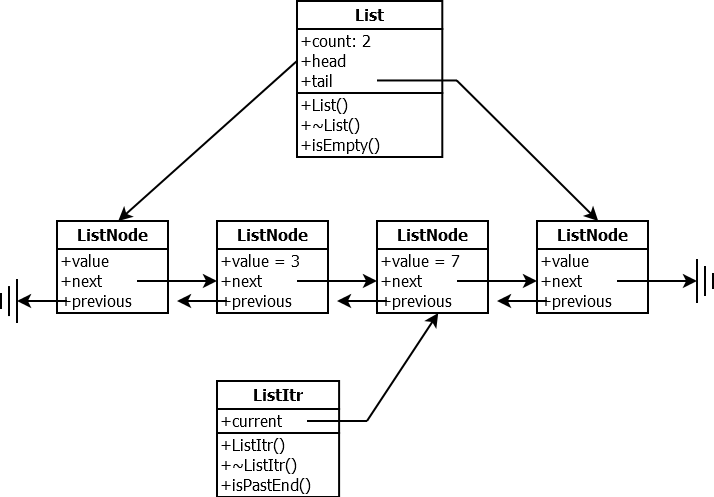
\includegraphics[height=0.9\textheight]{list-diagram}
\end{frame}

\begin{frame}[fragile,label=labListDecl]{the lab's list declaration}
\lstset{
    language=C++,
    style=small,
    moredelim={**[is][\btHL<all:2>]{@2}{2@}},
    moredelim={**[is][\btHL<all:3>]{@3}{3@}},
    moredelim={**[is][\btHL<all:4>]{@4}{4@}},
}
\begin{lstlisting}
class ListNode {

public:
    ListNode();                // Constructor
    ...
private:
    int value;
    @2ListNode *next, *previous2@;

    @3friend class List;3@
    @4friend class ListItr;4@
};
\end{lstlisting}
\begin{tikzpicture}[overlay,remember picture]
\coordinate (place) at ([yshift=4cm]current page.south);
\tikzset{
    markBox/.style={draw=red,very thick,align=left,at=(place), fill=white},
}
\begin{visibleenv}<2>
\node[markBox] {\texttt{*} binds to name --- declares two pointers; \\
                (why I write \texttt{*} next to names)};
\end{visibleenv}
\begin{visibleenv}<3>
\node[markBox] {the class \texttt{List} can access \\ private members of \texttt{ListNode}};
\end{visibleenv}
\begin{visibleenv}<4>
\node[markBox] {the class \texttt{ListItr} can access \\ private members of \texttt{ListNode}};
\end{visibleenv}
\end{tikzpicture}
\end{frame}

\begin{frame}[fragile,label=labListLocal]{a common mistake}
\lstset{
    language=C++,
    style=small,
    moredelim={**[is][\btHL<all:2>]{@2}{2@}},
    moredelim={**[is][\btHL<all:3>]{@3}{3@}},
    moredelim={**[is][\btHL<all:4>]{@4}{4@}},
}
\begin{lstlisting}
class Foo {
public:
  Foo();
private:
  ListNode *@2head2@;
  ...
};
Foo::Foo() {
  ListNode *@2head2@ = new ListNode; // BROKEN!
}
\end{lstlisting}
\begin{itemize}
\item what's wrong with this?
\end{itemize}
\begin{tikzpicture}[overlay,remember picture]
    \tikzset{
        >=Latex,
    }
\coordinate (place) at ([yshift=8cm,xshift=0cm]current page.south);
\begin{visibleenv}<2->
\node[draw,font=\tt,thick,anchor=north west,label={north:Foo object},minimum width=2cm] (fooHead) at (place) {
    head
};
\node[draw,font=\tt,thick,anchor=north west,minimum width=2cm] (fooRest) at (fooHead.south west) {\ldots};
    \node[draw,font=\tt,thick,anchor=north west,label={north:local variables}] (fooLocal) at ([yshift=-2.5cm]place) {
    head
};
\end{visibleenv}
\begin{visibleenv}<3->
    \node[right=1cm of fooHead,label={north:ListNode},rectangle split,rectangle split parts=3,draw] (fooNode) {
    next
    \nodepart{second} prev
    \nodepart{third} \ldots
};
    \draw[ultra thick,red,->] (fooLocal) -- ++(1cm,0cm) |- (fooNode)
\end{visibleenv}
\end{tikzpicture}
\end{frame}


% FIXME: missing topics:
    % dynamic allocation extra space

\section{dynamic memory allocation (2)}

\begin{frame}[fragile,label=memCpp]{memory.cpp}
\lstset{
    language=C++,
    style=smaller,
    moredelim={**[is][\btHL<all:1>]{@1}{1@}},
    moredelim={**[is][\btHL<all:2>]{@2}{2@}},
    moredelim={**[is][\btHL<all:3>]{@3}{3@}},
    moredelim={**[is][\btHL<all:4>]{@4}{4@}},
}
\begin{lstlisting}
class Foo { long x, y; };
int main() {
    cout << "sizeof(long): " << @2sizeof(long)2@ << endl;
    cout << "sizeof(Foo): " << @2sizeof(Foo)2@ << endl;
    Foo *quux = new Foo;
    Foo *bar = new Foo;
    long diff = @3((long)bar)-((long)quux)3@;
    cout << "First foo: " << @4bar4@ << endl;
    cout << "Second foo: " << quux << endl;
    cout << "Difference: " << diff << endl;
    delete quux; delete bar;
    return 0;
}
\end{lstlisting}
\begin{tikzpicture}[overlay,remember picture]
\coordinate (place) at ([yshift=2cm]current page.south);
\coordinate (place2) at ([yshift=3cm]current page.south);
\tikzset{
    markBox/.style={draw=red,very thick,align=left,at=(place), fill=white},
    markBoxB/.style={draw=red,very thick,align=left,at=(place2), fill=white},
}
\begin{visibleenv}<2>
\node[markBox] {{\tt sizeof} operator --- how many bytes is $X$?};
\end{visibleenv}
\begin{visibleenv}<3>
\node[markBox] {convert pointers to integers, subtract \\ = distance in memory};
\end{visibleenv}
\begin{visibleenv}<4>
\node[markBox] {prints out address};
\end{visibleenv}
\end{tikzpicture}
\end{frame}

\begin{frame}[fragile,label=memCppOut]{memory.cpp output}
One (of many) possible output:
\begin{Verbatim}
sizeof(long): 8
sizeof(Foo): 16
1st Foo: 0x1ec4030
2nd Foo: 0x1ec4050
Difference: 32
\end{Verbatim}
\begin{itemize}
\item 32 bytes apart? --- \myemph{16 extra bytes?}
\item implementation of \texttt{new} storing metadata
    \begin{itemize}
    \item need extra space \textit{somewhere} to track size, etc.
    \end{itemize}
\end{itemize}
\end{frame}


\section{references}

%\begin{comment}
\begin{frame}{last time}
    \begin{itemize}
    \item classes
        \begin{itemize}
        \item declarations in {\tt .h} file
        \item {\tt ClassName::method}
        \item {\tt class ... \{...\}\myemph{;}}
        \item {\tt const}, {\tt static}
        \end{itemize}
    \item objects --- values, not references
        \begin{itemize}
        \item {\tt return Foo(1)} --- {\tt Foo(1)} is temporary Foo object
        \item {\tt x = y} --- copy {\tt x} into {\tt y}
        \end{itemize}
    \item the preprocessor --- {\tt \#define}, {\tt \#include}, etc.
    \item started pointers
    \end{itemize}
\end{frame}
\end{comment}

\begin{comment}
\begin{frame}{last time}
    \begin{itemize}
    \item pointers
        \begin{itemize}
        \item memory --- array of bytes
        \item pointers --- indices into array --- addresses
        \item {\tt T *} --- pointer to T type
        \item {\tt *somePointer} --- use thing at address `pointed to'
        \item {\tt \&someVariable} --- address of someVariable
            \begin{itemize}
            \item AKA ``pointer to'' someVariable
            \end{itemize}
        \end{itemize}
    \item started {\tt new}/{\tt delete}
    \end{itemize}
\end{frame}
\end{comment}

\begin{comment}
\begin{frame}[fragile,label=lastTime]{last time}
\lstset{language=C++,style=small}
    \begin{itemize}
    \item arrays in C++
        \begin{itemize}
        \item \lstinline|int foo[100];|
        \item \lstinline|int *foo = new int[100]; ... delete[] foo;|
        \item \lstinline|foo[42]|
        \end{itemize}
    \item references
        \begin{itemize}
        \item \lstinline|int &refToX = x;|
        \item \lstinline|refToX = valueToAssignToX;|
        \item \lstinline|funcNeedingInt(refToX);|
        \item automatically dereferenced pointers
        \end{itemize}
    \item references as function arguments/pass (started)
    \end{itemize}
\end{frame}

\begin{frame}{SDAC note-taking assistence}
    \begin{itemize}
    \item Student Disability Access Center website ---
        \begin{itemize}
        \item \url{https://studenthealth.virginia.edu/sdac}
        \item ``Notetaker Application'' link
        \end{itemize}
    \end{itemize}
\end{frame}
\end{comment}

\begin{frame}[fragile,label=lastTime]{last time}
\lstset{language=C++,style=small}
    \begin{itemize}
    \item references to const
    \item default methods and destructors
        \begin{itemize}
            \item \lstinline|Foo::Foo()| --- default constructor
            \item \lstinline|Foo::Foo(const Foo& other)| --- copy constructor
            \item \lstinline|Foo::~Foo()| --- destructors
            \item \lstinline|Foo &Foo::operator=(const Foo& other)| --- assignment
        \end{itemize}
    \item overriding operators
        \begin{itemize}
            \item \lstinline|operator>>|, \lstinline|opreator<<| for \lstinline|cin|, \lstinline|cout|
            \item \lstinline|operator+|, \lstinline|operator+=| for \lstinline|string|
            \item \ldots
        \end{itemize}
    \item \lstinline|operator<<|, etc. as method or global function
    \end{itemize}
\end{frame}


% FIXME: hilight assignment
\begin{frame}[fragile,label=cppReferences]{C++ references}
\lstset{
    language=C++,
    style=small
}
\begin{lstlisting}
int x, y;
int &referenceToX = x;
x = 42; y = 100;
cout << referenceToX << " ";  // output: 42
referenceToX = y;  // sets x
cout << referenceToX << " ";  // output: 100
y = 99;
cout << x << " " << y;        // output: 100 99
\end{lstlisting}
\end{frame}

\begin{frame}{references}
    \begin{itemiz[e}
    \item \myemph{alternate name} for a value
    \item like pointers that are automatically dereferenced
    \item can only \myemph{bind} references at initialization
    \end{itemize}
\end{frame}

\begin{frame}[fragile,label=swapRef]{swap with references}
\lstset{
    language=C++,
    style=small
}
\begin{lstlisting}
void swapWithPointers(int *x, int *y) {
    int temp = *y;
    *y = *x;
    *x = temp;
}

void swapWithReferences(int &x, int &y) {
    int temp = y;
    y = x;
    x = temp;
}
\end{lstlisting}
\end{frame}

\begin{frame}[fragile,label=usingSwap]{using swap}
\lstset{
    language=C++,
    style=small
}
\begin{lstlisting}
int main(void) {
    int x = 42, y = 100;
    swapWithPointers(&x, &y);
    cout << x << " " << y << endl; 
        // output: 100 42

    x = 42; y = 100;
    swapWithReferences(x, y);
    cout << x << " " << y << endl; 
        // output: 100 42
    return 0;
}
\end{lstlisting}
\end{frame}

\begin{frame}[fragile,label=refToClass]{references to classes}
\begin{lstlisting}
class Square {
    ...
public:
    int sideLength;
};
...
Square *ptr = ...;
doSomethingWith(ptr->sideLength);
doSomethingWith((*ptr).sideLength);
Square &ref = ...;
doSomwthingWIth(ref.sideLength);
\end{lstlisting}
\end{frame}


\subsection{uses of \&}

\begin{frame}[fragile,label=confAmp]{\texttt{*} and \texttt{\&}}
\lstset{
    language=C++,
    style=small,
}
\begin{itemize}
    \item \lstinline|int *p = q| --- \begin{tabular}{l}p is a pointer to int\\ initially contains \textit{address} q\end{tabular}
\item \lstinline|&y| --- \begin{tabular}{l}
                                 pointer to y
                            \end{tabular}
\item \lstinline|int *p = &y; cout << *p| --- outputs y's value
\item \lstinline|int *p; p = &y; cout << *p| --- outputs y's value
    \hrule
\item \lstinline|int &r = y| --- \begin{tabular}{l}
                                    r is a reference to int \\
                                    bound to y
                                 \end{tabular}
\item \lstinline|int &r = y; cout << r| --- outputs y's value
\end{itemize}
\end{frame}


\subsection{pass-by-value}

\begin{comment}
\begin{frame}{last time}
    \begin{itemize}
    \item classes
        \begin{itemize}
        \item declarations in {\tt .h} file
        \item {\tt ClassName::method}
        \item {\tt class ... \{...\}\myemph{;}}
        \item {\tt const}, {\tt static}
        \end{itemize}
    \item objects --- values, not references
        \begin{itemize}
        \item {\tt return Foo(1)} --- {\tt Foo(1)} is temporary Foo object
        \item {\tt x = y} --- copy {\tt x} into {\tt y}
        \end{itemize}
    \item the preprocessor --- {\tt \#define}, {\tt \#include}, etc.
    \item started pointers
    \end{itemize}
\end{frame}
\end{comment}

\begin{comment}
\begin{frame}{last time}
    \begin{itemize}
    \item pointers
        \begin{itemize}
        \item memory --- array of bytes
        \item pointers --- indices into array --- addresses
        \item {\tt T *} --- pointer to T type
        \item {\tt *somePointer} --- use thing at address `pointed to'
        \item {\tt \&someVariable} --- address of someVariable
            \begin{itemize}
            \item AKA ``pointer to'' someVariable
            \end{itemize}
        \end{itemize}
    \item started {\tt new}/{\tt delete}
    \end{itemize}
\end{frame}
\end{comment}

\begin{comment}
\begin{frame}[fragile,label=lastTime]{last time}
\lstset{language=C++,style=small}
    \begin{itemize}
    \item arrays in C++
        \begin{itemize}
        \item \lstinline|int foo[100];|
        \item \lstinline|int *foo = new int[100]; ... delete[] foo;|
        \item \lstinline|foo[42]|
        \end{itemize}
    \item references
        \begin{itemize}
        \item \lstinline|int &refToX = x;|
        \item \lstinline|refToX = valueToAssignToX;|
        \item \lstinline|funcNeedingInt(refToX);|
        \item automatically dereferenced pointers
        \end{itemize}
    \item references as function arguments/pass (started)
    \end{itemize}
\end{frame}

\begin{frame}{SDAC note-taking assistence}
    \begin{itemize}
    \item Student Disability Access Center website ---
        \begin{itemize}
        \item \url{https://studenthealth.virginia.edu/sdac}
        \item ``Notetaker Application'' link
        \end{itemize}
    \end{itemize}
\end{frame}
\end{comment}

\begin{frame}[fragile,label=lastTime]{last time}
\lstset{language=C++,style=small}
    \begin{itemize}
    \item references to const
    \item default methods and destructors
        \begin{itemize}
            \item \lstinline|Foo::Foo()| --- default constructor
            \item \lstinline|Foo::Foo(const Foo& other)| --- copy constructor
            \item \lstinline|Foo::~Foo()| --- destructors
            \item \lstinline|Foo &Foo::operator=(const Foo& other)| --- assignment
        \end{itemize}
    \item overriding operators
        \begin{itemize}
            \item \lstinline|operator>>|, \lstinline|opreator<<| for \lstinline|cin|, \lstinline|cout|
            \item \lstinline|operator+|, \lstinline|operator+=| for \lstinline|string|
            \item \ldots
        \end{itemize}
    \item \lstinline|operator<<|, etc. as method or global function
    \end{itemize}
\end{frame}


\begin{frame}[fragile,label=arrowSyn]{reminder: re arrow syntax}
\lstset{
    language=C,
    style=small
}
\begin{lstlisting}
Rational r; r.num = 4;
Rational *p = new Rational;
(*p).num = 4;
(*p).print();
p->num = 4;  // "follow the pointer"
p->print();
Rational &ref = r;
ref.num = 4;
ref.print();
\end{lstlisting}
\end{frame}


\begin{frame}[fragile,label=cppValue1]{pass-by-value (1)}
    \lstset{language=C++,style=small}
\begin{lstlisting}
class IntWrapper { public: int value; };
void foo(IntWrapper arg) {
    arg.value = 42;
}
int main(void) {
    IntWrapper iw;
    iw.value = 100;
    foo(iw);
    cout << iw.value;
}
\end{lstlisting}
\begin{itemize}
    \item what is the output?
        \begin{tabular}{ll}
        A: 42  & C: crashes/doesn't compile \\
            \myemph<2->{\textbf<2->{B: 100}} & D: none of the above
        \end{tabular}
\end{itemize}
\end{frame}

\begin{frame}[fragile,label=cppValue2]{pass-by-value (2)}
\lstset{language=C++,style=small}
\begin{lstlisting}
class IntWrapper { public: int value; };
void foo(IntWrapper &arg) {
    arg.value = 42;
}
int main(void) {
    IntWrapper iw;
    iw.value = 100;
    foo(iw);
    cout << iw.value;
}
\end{lstlisting}
\begin{itemize}
    \item what is the output?
        \begin{tabular}{ll}
            \myemph<2>{\textbf<2->{A: 42}}  & C: crashes/doesn't compile \\
        B: 100 & D: none of the above
        \end{tabular}
\end{itemize}
\begin{tikzpicture}[overlay,remember picture]
\coordinate (place) at ([yshift=4cm,xshift=2cm]current page.south);
    \node[draw=red,thick] at (place) {
        \texttt{arg} bound to \texttt{iw}
};
\end{tikzpicture}
\end{frame}

\begin{frame}[fragile,label=cppValue3]{pass-by-value (3)}
\lstset{language=C++,style=small}
\begin{lstlisting}
class IntWrapper { public: int value; };
void foo(IntWrapper *arg) {
    arg.value = 42;
}
int main(void) {
    IntWrapper iw;
    iw.value = 100;
    foo(&iw);
    cout << iw.value;
}
\end{lstlisting}
\begin{itemize}
    \item what is the output?
        \begin{tabular}{ll}
            A: 42  &: \myemph<2->{\textbf<2->{C: crashes/doesn't compile}} \\
        B: 100 & D: none of the above
        \end{tabular}
    \item<3-> pointers don't have member variables
\end{itemize}
\end{frame}

\begin{frame}[fragile,label=cppValue4]{pass-by-value (4)}
\lstset{language=C++,style=small}
\begin{lstlisting}
class IntWrapper { public: int value; };
void foo(IntWrapper *arg) {
    arg->value = 42;  // same as:  (*arg).value = 42;
}
int main(void) {
    IntWrapper iw;
    iw.value = 100;
    foo(&iw);
    cout << iw.value;
}
\end{lstlisting}
\begin{itemize}
    \item what is the output?
        \begin{tabular}{ll}
            \myemph<2->{\textbf<2->{A: 42}}  & C: crashes/doesn't compile \\
        B: 100 & D: none of the above
        \end{tabular}
    \item<3-> pointer's value (address) is copied
\end{itemize}
\end{frame}

\begin{frame}[fragile,label=avoidingCopying]{avoiding copying}
\lstset{
    language=C++,
    style=small,
    moredelim={**[is][\btHL<all:2>]{@2}{2@}},
    moredelim={**[is][\btHL<all:3>]{@3}{3@}},
    moredelim={**[is][\btHL<all:4>]{@4}{4@}},
    moredelim={**[is][\btHL<all:5>]{@5}{5@}},
}
\begin{lstlisting}
@2bool lessThanCopy(Rational first, Rational second)2@ {
    return first.num * second.den < second.num * first.den;
}
@3bool lessThanNoCopy(const Rational &first,3@
                    @3const Rational &second)3@ {
    return first.num * second.den < second.num * first.den;
}
\end{lstlisting}
\begin{tikzpicture}
\begin{visibleenv}<2>
\node[draw,rectangle split,rectangle split parts=7,label={north:caller's memory}] (caller) {
    \ldots
    \nodepart{two} first.num
    \nodepart{three} first.den
    \nodepart{four} \ldots
    \nodepart{five} second.num
    \nodepart{six} second.den
    \nodepart{seven} \ldots
};
\node[right=1cm of caller,draw,rectangle split,rectangle split parts=4,label={north:lessThanCopy locals}] {
    first.num \nodepart{two}
    first.den \nodepart{three}
    second.num \nodepart{four}
    second.den
};
\end{visibleenv}
\begin{visibleenv}<3>
\node[draw,rectangle split,rectangle split parts=7,label={north:caller's memory}] (caller) {
    \ldots
    \nodepart{two} first.num
    \nodepart{three} first.den
    \nodepart{four} \ldots
    \nodepart{five} second.num
    \nodepart{six} second.den
    \nodepart{seven} \ldots
};
\node[right=3cm of caller,draw,rectangle split,rectangle split parts=2,label={north:lessThanNoCopy locals}] (nCLocal) {
    first
    \nodepart{two} second
};
\draw[-Latex,thick] (nCLocal.one west) -- (caller.two east);
\draw[-Latex,thick] (nCLocal.two west) -- (caller.five east);
\end{visibleenv}
\end{tikzpicture}
\end{frame}

\begin{frame}[fragile,label=constReferneces]{const}
\lstset{
    language=C++,
    style=smaller,
}
    \vspace{-.75cm}
\begin{lstlisting}
// no copy, modifies original 
void foo(Rational& value) { 
    value = Rational(4, 3);
}

// makes copy, modifies copy
void fooBroken1(Rational value) {  
    value = Rational(4, 3);  // BROKEN
}

// makes const(ant) copy, error modifying
void fooBroken1(const Rational value) { 
    value = Rational(4, 3);  // ERROR
}

// no copy, error modifying
void fooBroken2(const Rational& value) {
    value = Rational(4, 3);  // ERROR
}
\end{lstlisting}
\end{frame}

\begin{frame}[fragile,label=returnByRef]{return-by-reference}
\lstset{language=C++,style=small}
\begin{lstlisting}
int counter;  // global variable
int &get_counter_reference() {
    return counter;
}
...
get_counter_reference() = 42;
cout << get_counter_reference() << endl;  // output: 42
\end{lstlisting}
\end{frame}

\begin{frame}[fragile,label=returnByRefCaution]{return-by-reference --- caution}
\lstset{language=C++,style=small}
\begin{lstlisting}
int &get_counter_reference() {
    int counter = 0;
    return counter;   // ERROR
}
...
get_counter_reference() = 42; 
    // ERROR -- writing unallocated object
\end{lstlisting}
\end{frame}


\section{built-in methods}

\begin{frame}[fragile,label=implMeth]{implicit methods}
    \lstset{language=C++,style=small}
\begin{lstlisting}
class Foo {};
\end{lstlisting}
\begin{itemize}
    \item Foo has the following methods:
    \begin{itemize}
    \item \texttt{Foo()} --- default constructor
    \item \texttt{Foo(const Foo\&)} --- copy constructor
    \item \texttt{\textasciitilde{}Foo()} --- destructor
    \item \texttt{operator=(const Foo\&)} --- assignment operator
    \end{itemize}
    \item created by compiler, but you can override
\end{itemize}
\end{frame}

\begin{frame}[fragile,label=defaultConstructor]{default constructor/destructor}
\lstset{language=C++,style=small}
\begin{tikzpicture}
\node[] (foo) {
\begin{lstlisting}
class Foo { public: Foo(); ~Foo(); };
Foo::Foo() { cout << "Foo::Foo()" << endl; }
Foo::~Foo() { cout << "Foo::~Foo()" << endl; }
int main() {
    Foo local; 
    cout << "(1)\n";
    Foo *ptr = new Foo;  
    cout << "(2)\n";
    delete ptr;
    cout << "(3)\n";
    return 0;
};
\end{lstlisting}
};
    \node[draw,thick,anchor=north west,align=left] at ([xshift=7.75cm,yshift=-2cm]foo.north west) {
\lstset{language={}}
output: \\
\begin{lstlisting}
Foo::Foo()
(1)
Foo::Foo()
(2)
Foo::~Foo()
(3)
Foo::~Foo()
\end{lstlisting}
};
\end{tikzpicture}
\end{frame}

\begin{frame}[fragile,label=whyDestructor]{why destructors}
\lstset{language=C++,style=small}
\begin{tikzpicture}
\node[] (foo) {
\begin{lstlisting}
class DynamicArray {
    ...
    ~DynamicArray();
private:
    int *pointer;  // allocated with new int[...]
};
...
DynamicArray::~DynamicArray() {
    delete[] pointer;
}
\end{lstlisting}
};
\end{tikzpicture}
\end{frame}

\begin{frame}[fragile,label=copyConstructor1]{copy constructors, operator=  (1)}
\lstset{language=C++,style=small}
\begin{tikzpicture}
\node[] (foo) {
\begin{lstlisting}
Foo a, b;

// invokes Foo::Foo(const Foo&)
Foo copy1(a);   

// invokes Foo::Foo(const Foo&)
Foo copy2 = a;

// invokes Foo::operator=(const Foo&);
b = a;
\end{lstlisting}
};
\end{tikzpicture}
\end{frame}

\begin{frame}[fragile,label=exampleCCOpEq]{default implementations}
\lstset{language=C++,style=smaller}
    \vspace{-.75cm}
\begin{tikzpicture}
\node[] (foo) {
\begin{lstlisting}
// equivalent to default implementation:
Rational::Rational(const Rational &other) {
    // copy all member variables
    den = other.den;
    num = other.num;
}

// equivalent to default implementation:
Rational &Rational::operator=(
        const Rational &other) {
    // copy all members
    den = other.den;
    num = other.num;
    // return reference to this so
    //    foo = bar = baz 
    // works
    return *this;
}
\end{lstlisting}
};
\end{tikzpicture}
\end{frame}


\section{operator overloading}

\begin{frame}[fragile,label=opOverload1]{operator=}
\lstset{language=C++,style=smaller}
\begin{lstlisting}
class Foo { public:
    Foo& operator=(const Foo& other);
}
Foo & Foo::operator=(const Foo& other) {
    cout << "called Foo::operator=";
    return *this;
}
int main() {
    Foo x, y;
    x = y;  // output:  called Foo::operator=
}
\end{lstlisting}
\end{frame}

\begin{frame}[fragile,label=opOverload2]{overrided operators can do whatever}
\lstset{language=C++,style=smaller}
\begin{lstlisting}
class Bar {};
class Foo { public:
    Foo();
    Foo& operator=(const Bar& other);
    int count;
}
Foo::Foo() : count(0) {}
Foo & Foo::operator=(const Bar& other) {
    cout << "count=" << ++count;
    return *this;
}
int main() {
    Foo x;
    x = Bar();
        // output count=1
    x = Bar();
        // output count=2
}
\end{lstlisting}
\end{frame}


\begin{frame}[fragile,label=opOverExs]{more operator overriding (1)}
\lstset{language=C++,style=smaller}
\begin{lstlisting}
    // ostream &ostream::operator<<(const char*)
cout << "Foo" << endl;
    // istream &istream::operator>>(int&)
cin >> number;
\end{lstlisting}
\hrule
\begin{lstlisting}
#include <string>
using std::string;
...
    // string::string(const char*)
string x = "This is the first part.";
string y = " And this is the second part.";

    // string string::operator+(const string&) const
string y = x + z;

    // string &string::operator+=(const char*)
y += " And this is the third part.";
\end{lstlisting}
\end{frame}

\begin{frame}[fragile,label=opOverExs2]{more operator overloading (2)}
\begin{lstlisting}
class Rational {
    ...
    Rational operator*(const Rational& other)
        const;
    Rational operator+(const Rational& other)
        const;
    ...
};
Rational x(2, 4), y(4, 5);
Rational z = x * y + y;
\end{lstlisting}
\end{frame}

\begin{frame}[fragile,label=opImplMeth]{operator overloading with methods}
\lstset{language=C++,style=smaller}
\begin{lstlisting}
int x = 42;
cout << "The value is: " << x << endl;
// same as:
cout.operator<<("The value is: ").operator<<(x).operator<<(endl);
\end{lstlisting}
\hrule
\begin{lstlisting}
/* approximate code ... */
class ostream {
    ...
    ostream &operator<(int value);
};
...
ostream &ostream::operator<<(int value) {
    ...
    return *this;
}
\end{lstlisting}
\end{frame}

\begin{frame}[fragile,label=opImplFunc]{operator overloading with functions}
\lstset{language=C++,style=smaller}
\begin{lstlisting}
#include <string>
using std::cout; using std::string;
...
string x = ...;  // like Java String class
cout << x;
// same as:
operator<<(cout, x);
\end{lstlisting}
\hrule
\begin{lstlisting}
ostream& operator<<(ostream& out, const string &s) {
    ...
    return out;
}
\end{lstlisting}
\end{frame}


\section{advanced classes example}

\begin{frame}[fragile,label=overExOver]{C++ combined example}
    \begin{itemize}
    \item test class to demo constructors, operator=, etc.
    \item single file with all examples for test class: cpptest.cpp
    \item this lecture: in independent pieces
    \end{itemize}
\end{frame}


\begin{frame}[fragile,label=overEx]{C++ combined example (test.h)}
\lstset{
    language=C++,
    style=smaller,
    moredelim={**[is][\btHL<all:2>]{@2}{2@}},
    moredelim={**[is][\btHL<all:3>]{@3}{3@}},
    moredelim={**[is][\btHL<all:4>]{@4}{4@}},
}
\begin{lstlisting}
// test.h:
class test {
    static int idcount;
    @2const2@ int id;
    int value;
  public:
    test();
    test(int v);
    test(const test& x);
    ~test();
    test& operator=(const test& other);
    friend @3ostream& operator<<3@(ostream& out,
                                 const test& f);
};
\end{lstlisting}
\begin{tikzpicture}[overlay,remember picture]
\coordinate (place) at ([yshift=5cm,xshift=2cm]current page.south);
\tikzset{
    box/.style={draw=red,very thick,at=(place),fill=white,align=left},
}
    \begin{visibleenv}<2>
        \node[box] {\texttt{const} --- must be set in constructor};
    \end{visibleenv}
    \begin{visibleenv}<3>
        \node[box] {friend function for \\ outputting to an ostream (like cout)};
    \end{visibleenv}
\end{tikzpicture}
\end{frame}

\begin{frame}[fragile,label=overEx2]{C++ combined example (test.cpp)}
\lstset{
    language=C++,
    style=smaller,
    moredelim={**[is][\btHL<all:2>]{@2}{2@}},
    moredelim={**[is][\btHL<all:3>]{@3}{3@}},
    moredelim={**[is][\btHL<all:4>]{@4}{4@}},
}
\begin{lstlisting}
// test.cpp:
@2int test::idcount = 0;2@

ostream &operator<<(ostream &out, const test &f) {
  out << "test[id=" << f.id << ",v="
      << f.value << "]@" << &f;
  return out;
}

test::test(const test& x) : id(x.id), @3value(x.value)3@ {
  cout << "calling test(" << x <<"); object created is " << *this << endl;
}

test &@4test::operator=4@(const test &other) {
  cout << "calling " << *this
       << ".operator=(" << other << ")" << endl;
  return *this;
}
/* and similar for constructors */
\end{lstlisting}
\begin{tikzpicture}[overlay,remember picture]
\coordinate (place) at ([yshift=5cm,xshift=1cm]current page.south);
\tikzset{
    box/.style={draw=red,very thick,at=(place),align=left,fill=white},
}
    \begin{visibleenv}<2>
        \node[box] {\lstinline|class test { static int idcount; ... }|};
    \end{visibleenv}
    \begin{visibleenv}<3>
        \node[box] {\texttt{const}, so must be \\ on initialization list};
    \end{visibleenv}
    \begin{visibleenv}<4>
        \node[box] {called like assignment doesn't actually assign!};
    \end{visibleenv}
\end{tikzpicture}
\end{frame}

% FIXME: show constructors?

\begin{frame}[fragile,label=testtrivial]{trivial test object: testtrivial.cpp}
\lstset{
    language=C++,
    style=smaller,
    moredelim={**[is][\btHL<all:2>]{@2}{2@}},
    moredelim={**[is][\btHL<all:3>]{@3}{3@}},
    moredelim={**[is][\btHL<all:4>]{@4}{4@}},
}
\begin{lstlisting}
int main() {
    cout << "about to create aa" << endl;
    @2test aa;2@
    cout << "aa is: " << aa << endl;
    @3return 0;3@
}
\end{lstlisting}
\hrule
    \lstset{language={},style=smaller,
    moredelim={**[is][\btHL<all:2>]{@2}{2@}},
    moredelim={**[is][\btHL<all:3>]{@3}{3@}},
    moredelim={**[is][\btHL<all:4>]{@4}{4@}},
    }
\begin{lstlisting}
about to create aa
@2calling test(); object created is2@
     @2test[id=0,v=0]@0x7ffc82ba94402@
aa is: test[id=0,v=0]@0x7ffc82ba9440
@3calling ~test() on test[id=0,v=0]@0x7ffc82ba94403@
\end{lstlisting}
\end{frame}

\begin{frame}[fragile,label=usingTest2]{trivial test object: testint.cpp}
\lstset{
    language=C++,
    style=smaller,
    moredelim={**[is][\btHL<all:2>]{@2}{2@}},
    moredelim={**[is][\btHL<all:3>]{@3}{3@}},
    moredelim={**[is][\btHL<all:4>]{@4}{4@}},
}
\begin{lstlisting}
int main() {
    cout << "about to create b" << endl;
    @2test b(1);2@
    cout << "b is: " << b << endl;
    return 0;
}
\end{lstlisting}
\hrule
    \lstset{language={},style=smaller,
    moredelim={**[is][\btHL<all:2>]{@2}{2@}},
    moredelim={**[is][\btHL<all:3>]{@3}{3@}},
    moredelim={**[is][\btHL<all:4>]{@4}{4@}},
    }
\begin{lstlisting}
about to create aa
@2calling test(); object created is2@
    @2test[id=0,v=0]@0x7ffed5659d702@
aa is: test[id=0,v=0]@0x7ffed5659d70
calling ~test() on test[id=0,v=0]@0x7ffed5659d70
\end{lstlisting}
\end{frame}

\begin{frame}[fragile,label=gotcha]{Type foo(): not a constructor call}
\lstset{
    language=C++,
    style=smaller,
    moredelim={**[is][\btHL<all:2>]{@2}{2@}},
    moredelim={**[is][\btHL<all:3>]{@3}{3@}},
    moredelim={**[is][\btHL<all:4>]{@4}{4@}},
}
\begin{lstlisting}
int main() {
    cout << "before test a()" << endl;
    test a();
    cout << "a is: " << a << endl;
    return 0;
}
\end{lstlisting}
\hrule
``a is: 1''
\end{frame}

\begin{frame}[fragile,label=gotchaWarnings]{Type foo(): warnings}
\lstset{language={},style=smaller,
    moredelim={**[is][\btHL<all:2>]{@2}{2@}},
    moredelim={**[is][\btHL<all:3>]{@3}{3@}},
    moredelim={**[is][\btHL<all:4>]{@4}{4@}},
    }
\begin{lstlisting}
$ clang++ -Wall -pedantic -o testgotcha \
                 testgotcha.cpp test.cpp -I.
testgotcha.cpp:7:11: warning: empty parentheses
                    interpreted as a function
                    declaration [-Wvexing-parse]
    test a();
          ^~
testgotcha.cpp:7:11: note: remove parentheses to
                     declare a variable
    test a();
          ^~
testgotcha.cpp:8:25: warning: address of function 'a'
                     will always evaluate to 'true'
                     [-Wpointer-bool-conversion]
    cout << "a is: " << a << endl;
\end{lstlisting}
\end{frame}

\begin{frame}[fragile,label=testnew]{new}
\lstset{
    language=C++,
    style=smaller,
    moredelim={**[is][\btHL<all:2>]{@2}{2@}},
    moredelim={**[is][\btHL<all:3>]{@3}{3@}},
    moredelim={**[is][\btHL<all:4>]{@4}{4@}},
}
\begin{lstlisting}
int main() {
    test *c = new test(2);
    cout << "created *c: " << *c << endl;
    test *d = new test;
    cout << "created *d: " << *d << endl;
    @2return 0;2@
}
\end{lstlisting}
\hrule
\lstset{language={},style=smaller,
    moredelim={**[is][\btHL<all:2>]{@2}{2@}},
    moredelim={**[is][\btHL<all:3>]{@3}{3@}},
    moredelim={**[is][\btHL<all:4>]{@4}{4@}},
    }
\begin{lstlisting}
calling test(2); object created is test[id=0,v=2]@0x144dc20
created *c: test[id=0,v=2]@0x144dc20
calling test(); object created is test[id=1,v=0]@0x144e050
created *d: test[id=1,v=0]@0x144e050
\end{lstlisting}
\end{frame}

\begin{frame}[fragile,label=testnew]{new + delete}
\lstset{
    language=C++,
    style=smaller,
    moredelim={**[is][\btHL<all:2>]{@2}{2@}},
    moredelim={**[is][\btHL<all:3>]{@3}{3@}},
    moredelim={**[is][\btHL<all:4>]{@4}{4@}},
}
\begin{lstlisting}
int main() {
    test *c = new test(2);
    test *d = new test;
    delete c;
    return 0;
}
\end{lstlisting}
\hrule
\lstset{language={},style=smaller,
    moredelim={**[is][\btHL<all:2>]{@2}{2@}},
    moredelim={**[is][\btHL<all:3>]{@3}{3@}},
    moredelim={**[is][\btHL<all:4>]{@4}{4@}},
    }
\begin{lstlisting}
calling test(2); object created is test[id=0,v=2]@0xe91c20
calling test(); object created is test[id=1,v=0]@0xe92050
calling ~test() on test[id=0,v=2]@0xe91c20
\end{lstlisting}
\end{frame}

% FIXME: copy constructor


\begin{frame}[fragile,label=testbar]{function call}
\lstset{
    language=C++,
    style=smaller,
    moredelim={**[is][\btHL<all:2>]{@2}{2@}},
    moredelim={**[is][\btHL<all:3>]{@3}{3@}},
    moredelim={**[is][\btHL<all:4>]{@4}{4@}},
}
\begin{lstlisting}
test bar(@2test param2@) {
  return test(10);
}
int main() {
  test *c = new test(2);  // oops: never deleted
  cout << "about to call bar" << endl;
  test e = bar(@2*c2@);
  cout << "done calling bar" << endl;
}
\end{lstlisting}
\hrule
\lstset{language={},style=smaller,
    moredelim={**[is][\btHL<all:2>]{@2}{2@}},
    moredelim={**[is][\btHL<all:3>]{@3}{3@}},
    moredelim={**[is][\btHL<all:4>]{@4}{4@}},
    }
\begin{lstlisting}
calling test(2); object created is test[id=0,v=2]@0x17b1c20
about to call bar
calling test(@2test[id=0,v=2]@0x17b1c202@); object created is test[id=0,v=2]@@20x7ffcea9375282@
calling @3test(10); object created is test[id=1,v=10]@0x7ffcea9375303@
calling ~test() on test[id=0,v=2]@@20x7ffcea9375282@
done calling bar
calling ~test() on @3test[id=1,v=10]@0x7ffcea9375303@
\end{lstlisting}
\begin{tikzpicture}[overlay,remember picture]
\coordinate (place) at ([yshift=5cm,xshift=1cm]current page.south);
\tikzset{
    box/.style={draw=red,very thick,at=(place),align=left,fill=white},
}
    \begin{visibleenv}<3>
        \node[box] {return value optimization: \\
                    compiler omitted copy constructor call \\
                    (but could have included it)};
    \end{visibleenv}
\end{tikzpicture}
\end{frame}

